%% LyX 2.1.2 created this file.  For more info, see http://www.lyx.org/.
%% Do not edit unless you really know what you are doing.
\documentclass[12pt,a4paper,english,portrait]{scrbook}
\usepackage[T1]{fontenc}
\usepackage[latin1]{inputenc}
\pagestyle{headings}
\setcounter{secnumdepth}{3}
\setcounter{tocdepth}{3}
\usepackage{color}
\usepackage{babel}
\usepackage{array}
\usepackage{varioref}
\usepackage{calc}
\usepackage{textcomp}
\usepackage{amsmath}
\usepackage{makeidx}
\makeindex
\usepackage{graphicx}
\usepackage[unicode=true,
 bookmarks=true,bookmarksnumbered=false,bookmarksopen=false,
 breaklinks=true,pdfborder={0 0 0},backref=false,colorlinks=true]
 {hyperref}
\hypersetup{pdftitle={CanReg5 - Instructions},
 pdfauthor={Morten Johannes ERVIK},
 pdfsubject={How to set up, run and work with CanReg5},
 pdfkeywords={CanReg5, Cancer registration}}

\makeatletter

%%%%%%%%%%%%%%%%%%%%%%%%%%%%%% LyX specific LaTeX commands.
\pdfpageheight\paperheight
\pdfpagewidth\paperwidth

%% Because html converters don't know tabularnewline
\providecommand{\tabularnewline}{\\}

%%%%%%%%%%%%%%%%%%%%%%%%%%%%%% Textclass specific LaTeX commands.
\newenvironment{lyxcode}
{\par\begin{list}{}{
\setlength{\rightmargin}{\leftmargin}
\setlength{\listparindent}{0pt}% needed for AMS classes
\raggedright
\setlength{\itemsep}{0pt}
\setlength{\parsep}{0pt}
\normalfont\ttfamily}%
 \item[]}
{\end{list}}

%%%%%%%%%%%%%%%%%%%%%%%%%%%%%% User specified LaTeX commands.
%% ================================================================================
%% This LaTeX file was created by AbiWord.                                         
%% AbiWord is a free, Open Source word processor.                                  
%% More information about AbiWord is available at http://www.abisource.com/        
%% ================================================================================
\usepackage{calc}\usepackage{fixltx2e}\usepackage{multicol}\usepackage[normalem]{ulem}%% Please revise the following command, if your babel
%% package does not support English (US)
\@ifundefined{definecolor}
 {\usepackage{color}}{}
\usepackage{hyperref}
\usepackage{breakurl}
\usepackage{listings}
\definecolor{lightyellow}{RGB}{255,255,200}
%% \lfoot{\today}

\makeatother

\usepackage{listings}
\begin{document}
\begin{center}

\includegraphics[width=0.66\columnwidth]{LogoBetaNewer}
\par\end{center}

\begin{center}
\textbf{Open Source}
\par\end{center}

\begin{center}
By: Morten Johannes Ervik, IARC 
\par\end{center}

\begin{center}
Version: \today\thispagestyle{empty}
\par\end{center}

\newpage{}

\tableofcontents{}

\newpage{}


\part{Introduction}


\chapter{What is CanReg?}

\begin{flushleft}
CanReg5 is an open source tool to input, store, check and analyse
cancer registry data. It has modules to do data entry, quality control,
consistency checks and basic analysis of the data. The main improvements
from the previous version are the new database engine, the improved
multi user capacities and that the development is managed like an
open source project. Also included is a tool to facilitate the set
up of a new or modification of an existing database by adding new
variables, tailoring the data entry forms etc. 
\par\end{flushleft}

\begin{flushleft}
Version 5 of CanReg is now ready for download.
\par\end{flushleft}


\section{A short introduction to the database structure in CanReg5\label{sub:A-short-introduction}}

\begin{flushleft}
New in CanReg5 is the three level table structure. Where CanReg4\index{CanReg4}
stored everything in one big table of tumours, CanReg5 splits this
information in three tables: Patient, Tumour and Source. For each
patient, you can store as many tumour records as you need, and for
each tumour you can store as many source records as you need. This
allows us to do more with our databases, for example related to completeness
by counting number of sources, but it poses come problem that might
require manual intervention during the conversion process of a system
from CanReg4 to CanReg5. 
\par\end{flushleft}

\begin{flushleft}
For example, some of you might store multiple sources in each tumour
record in CanReg4. This should be split into several source records
for this tumour record in CanReg5, but this is not an easy task to
automate since all registries that have opted for this have solved
it in a different way in CanReg4. 
\par\end{flushleft}

\begin{flushleft}
One way around this is to put all the fields related to the source
table in CanReg5 so that you are sure not to loose any data, and then
start from the date you start using CanReg5 to store multiple source
records per tumour. 
\par\end{flushleft}

\begin{flushleft}
The best way, but a more time consuming one, is to set up the source
table (by editing the system definition XML\index{XML}) to only contain
the data you want to store per source and then work on the exported
file from CanReg4 and import additional source information at a later
stage. (General import of data is not yet functioning adequately in
CanReg5 - only import \& migration of old data.) 
\par\end{flushleft}

\begin{flushleft}
You can of course choose not to use the source table, as well - just
record the source information per tumour like you would in CanReg4.
This can be set up while migrating your system definition files.
\par\end{flushleft}


\section{Forum\index{forum}, Issue tracker\index{issue tracker}, community
site\index{community site@community\textsf{\textbf{ }}site}, twitter\index{twitter}}

\begin{flushleft}
We have created a project page at SourceForge to help us keep track
of issues with CanReg5: \href{http://sourceforge.net/projects/canreg/}{http://sourceforge.net/projects/canreg/}.
Using tools there allows you to see what error reports other CanReg
users have already filed and if solutions have already been proposed
and also discuss potential improvements for CanReg5, before posting
your own queries.
\par\end{flushleft}

\begin{flushleft}
You can of course still send us emails at \href{mailto:canreg@iarc.fr}{canreg@iarc.fr}.
\par\end{flushleft}

\begin{flushleft}
If you encounter any problems please provide a description of it along
with the specifications of your computer. (Operating System (Windows
XP, Vista, 7, OSX, Linux?), memory, processor speed etc.) Also it
would be very useful if you can precise the \textbf{version\index{version}}
and the\textbf{ build code\index{build code}} of your CanReg5. This
can be found on the bottom left of the welcome screen and on the ``About''
screen. (For example Version: ``4.99.0b586'') 
\par\end{flushleft}

\begin{flushleft}
Please be aware that some problems can be avoided by installing the
latest version of the Java Runtime Environment (Version 6) before
you start. (Available from \href{http://java.com/en/download/manual.jsp}{http://java.com/en/download/manual.jsp}.) 
\par\end{flushleft}

\begin{flushleft}
Videos documenting certain operations described below can be downloaded
from: \href{http://www.iacr.com.fr/CanReg5/videos.zip}{http://www.iacr.com.fr/CanReg5/videos.zip}
. 
\par\end{flushleft}

\begin{flushleft}
Last, but not, least: CanReg has its own stream on twitter. Please
follow: \href{http://twitter.com/canreg}{http://twitter.com/canreg}
for updates. 
\par\end{flushleft}


\section{Getting hold of the latest version\index{latest version} of CanReg}

\begin{flushleft}
If you are running version 4.99.1 (or newer) of CanReg, you can launch
CanReg and click ``Options...'', go to the ``Advanced'' tab. (See
There you see your current version, i.e. 4.99.1. If you click ``Check''
CanReg will look for an updated version. Afterwards you can click
``Download latest version'' to get the zip-file containing the most
recent version of CanReg5. 
\par\end{flushleft}

\begin{figure}[h]
\begin{centering}
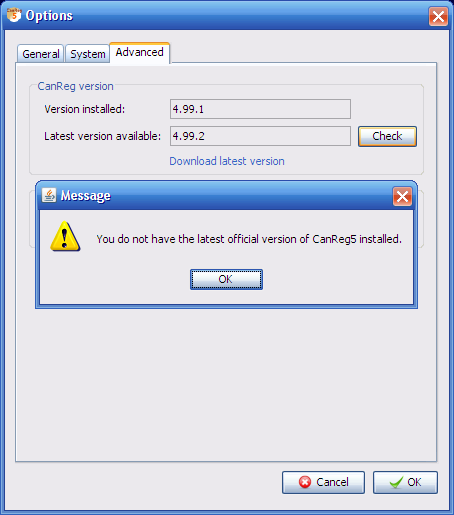
\includegraphics[width=4.72917in,height=5.36458in]{1}
\par\end{centering}

\protect\caption{Checking if you have the latest version of CanReg installed.}


\end{figure}


\begin{flushleft}
(If you have version 4.99.0 or no CanReg5 at all you can \index{download}download
the newest version from here: \href{http://www.iacr.com.fr/CanReg5/CanReg5.zip}{http://www.iacr.com.fr/CanReg5/CanReg5.zip})
\par\end{flushleft}


\section{Logfile}

\begin{flushleft}
CanReg generates a \index{logfile}logfile when you run it. This file
is called \index{canreg5client.log}canreg5client.log and is located
in your home folder. (On windows it is most probably under C:\textbackslash{}Documents
and Settings\textbackslash{}<your username> - you can access this
by browsing to \%HOMEPATH\% Depending on how you have configured your
computer it might show up as canreg5client.) If you can attach this
to emails with feedback/queries it would be very useful. Please note
that this file is overwritten each time CanReg is started, so you
need to ``take it'' just after, for example, your error occurs.
\par\end{flushleft}

\begin{flushleft}
\begin{minipage}[t]{1\columnwidth}%
Example content of a log-file:
\begin{lyxcode}
<?xml~version=\textquotedbl{}1.0\textquotedbl{}~encoding=\textquotedbl{}windows-1252\textquotedbl{}~standalone=\textquotedbl{}no\textquotedbl{}?>

<!DOCTYPE~log~SYSTEM~\textquotedbl{}logger.dtd\textquotedbl{}>

<log>

<record>
\begin{lyxcode}
<date>2009-06-25T16:09:27</date>

<millis>1245938967921</millis>

<sequence>0</sequence>

<logger>canreg.client.CanRegClientApp</logger>

<level>INFO</level>

<class>canreg.client.CanRegClientApp</class>

<method>startup</method>

<thread>10</thread>

<message>CanReg~version:~4.99.9b668~(20090625160546)</message>
\end{lyxcode}
</record>

...

</log>\end{lyxcode}
%
\end{minipage}
\par\end{flushleft}

\newpage{}


\part{Installing and running CanReg5\label{sec:Installing-and-running}}


\chapter{Software installation\index{installation}\index{software installation}}


\section{\label{sub:Java-Runtime-Environment}Install a recent Java Runtime
Environment\index{Java Runtime Environment@Java\textbf{ }Runtime\textbf{ }Environment}
\index{JRE}}

\begin{flushleft}
Before you install and run CanReg5 for the first time it is recommended
that you install the latest Java 7 Runtime Environment (April 2013:
Version 7 Update 21 ) You can get that from here: \href{http://java.com/en/download/manual.jsp}{http://java.com/en/download/manual.jsp}
\par\end{flushleft}


\section{\label{sub:Install-CanReg5}Install CanReg5}

CanReg5 is compatible with most major operating systems and the default
distribution of CanReg is simply a zip-archive.


\subsection{From CanReg5.zip}

\begin{flushleft}
To install it simply extract the content to a new folder, for example
on your desktop. (It is important to keep the same directory structure
as inside the zip-file.) 
\par\end{flushleft}

If you have tools like 7-zip or WinRar installed it is just a matter
of copying/moving the zip-file to the folder you want CanReg to reside,
right-clicking it and choose ``Extract here...'' 


\subsection{From CanReg5-Setup.zip (Windows only)}

An alternative way to install CanReg is by running the CanReg5-Setup.exe
from within CanReg5-Setup.zip. This is a standard windows installer
that will install CanReg5 in your ``Program Files'' folder (by default).
It is just a matter of clicking ``next'' ,''next'', ``next''
etc.


\section{Recommended Third Party tools}

It is recommended that you also install the following third party
software:


\subsection{Any post script viewer}

CanReg can produce tables in the post script format. To view these
you need a post script viewer like GhostView. (See \vref{sub:PostScript-Viewer}.)


\subsection{R }

Some of the more advanced analytical features in CanReg relies on
the free software called R. Please install this if you need to use
that functionality. (See \vref{sub:R}.) As of version 5.00.31, CanReg5
has a built in offline R package installer that can be installed in
parallell with CanReg5 and called from CanReg5 using the menu option
``Tools''->''Install R packages''. (This is only visible if you
have installed the R package installer.)


\section{Un-install\index{un-install} CanReg5}

\begin{flushleft}
If you wish to un-install CanReg5, delete the following folders (or
rename if you have anything valuable in them):\\
.CanRegClient\index{.CanRegClient} and .CanRegServer\index{.CanRegServer}
in your user folder.
\par\end{flushleft}

(On Windows you can get to your user folder\index{user folder} by
pressing Windows Key + R and then entering \%UserProfile\% and click
OK. See \url{http://en.wikipedia.org/wiki/Home_directory} for more
information.)

Afterwards you can delete the folder from \ref{sub:Install-CanReg5}.


\chapter{First launch}


\section{Run\index{run@\textsf{\textbf{run}}} CanReg5}

\begin{flushleft}
Go to the folder you installed CanReg5 in and double click on the
coffee cup icon (CanReg.jar). (\textbf{If, at this point, CanReg5
does not start you might have to update your Java Runtime Environment
and retry}. (See \vref{sub:Java-Runtime-Environment}.) 
\par\end{flushleft}

\begin{flushleft}
You should now be presented with the CanReg5 welcome window (See figure
\ref{fig:The-welcome-window}).
\par\end{flushleft}

\begin{center}
\begin{figure}[h]
\begin{centering}
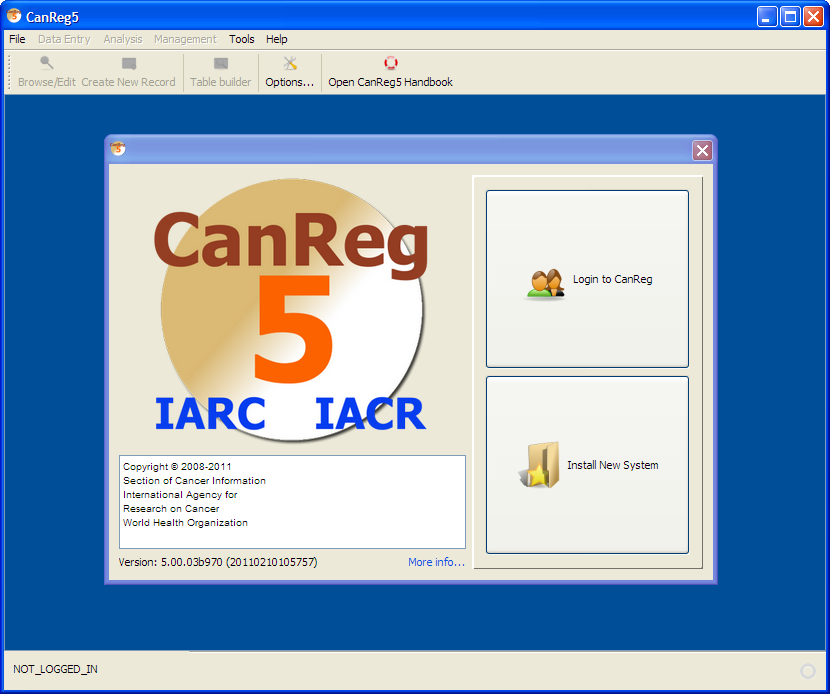
\includegraphics[width=0.9\linewidth]{CanRegWelcomeScreen}
\par\end{centering}

\protect\caption{\label{fig:The-welcome-window}The welcome window}


\end{figure}

\par\end{center}


\section{\index{demo system}Demo system}

\begin{flushleft}
Included is the dictionary for the training system located in the
demo-folder in the zip-file. With this you can get a demo-system up
and running to test some data entry. To run this demo system, install
the TRN-file to set up the system. Afterwards you should import the
dictionary using ``Data Entry'' - ''Edit dictionary'' and ``Import
complete dictionary from a file'', before you start to enter data. 
\par\end{flushleft}


\section{Install a new CanReg5 system\label{sub:Install-a-new}}

\begin{flushleft}
If you want to install an already provided system definition (for
example the demo system\index{demo system} TRN) please click ``Install
New System''. CanReg5 will present you with the following message:
\par\end{flushleft}

\begin{center}
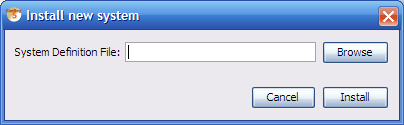
\includegraphics[width=4.20833in,height=1.30208in]{3}
\par\end{center}

\begin{flushleft}
Click browse to find the system definition file. (If you want to use
the TRN demo system look in demo/database and select TRN.xml and click
open and then Install.) 
\par\end{flushleft}

If the XML file is associated with a backup of CanReg5 the program
will ask you if you want to restore from this backup. 

\begin{center}
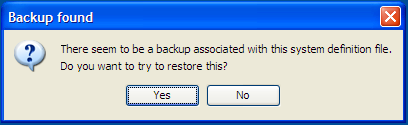
\includegraphics{backupdetected}
\par\end{center}

If you click yes CanReg will launch the server with the newly installed
system definitions and restore this backup. 


\section{Convert the CanReg4 system definitions}

\begin{flushleft}
If you have a CanReg4\index{CanReg4} system you can use tools built
into CanReg to help you migrate\index{migrate} this to CanReg5. 
\par\end{flushleft}

\begin{flushleft}
First import the variables of CanReg4 to CanReg5 - the system definition
of CanReg4. 
\par\end{flushleft}

\begin{flushleft}
Go to ``Tool'' in CanReg5 menu and click ``Convert system definition''
(See figure \vref{fig:CanReg-systems-definition-menu}.)
\par\end{flushleft}

\begin{center}
\begin{figure}
\begin{centering}
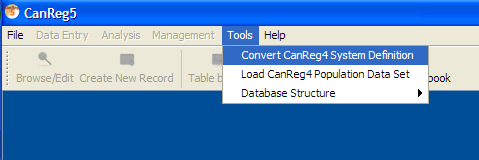
\includegraphics{4}
\par\end{centering}

\protect\caption{\label{fig:CanReg-systems-definition-menu}CanReg systems definition
converter menu}


\end{figure}

\par\end{center}

\begin{flushleft}
Do ``Browse'' to find your CanReg4 system definition file. (This
is a file located in the folder \textbackslash{}\textbackslash{}CR4SHARE\textbackslash{}CANREG4\textbackslash{}CR4-SYST\textbackslash{}
followed by your 3 letter registry code i.e. TRN whose name is ending
in .DEF (i.e. CR4-TRN.DEF).) 
\par\end{flushleft}

\begin{flushleft}
Select your CanReg4 file and double click it or click ``Open''. 
\par\end{flushleft}

\begin{flushleft}
Click ``Convert''. 
\par\end{flushleft}

\begin{flushleft}
The program will then ask you if you want to add this server to your
favourites. Click ``Yes'' here.
\par\end{flushleft}

\begin{center}
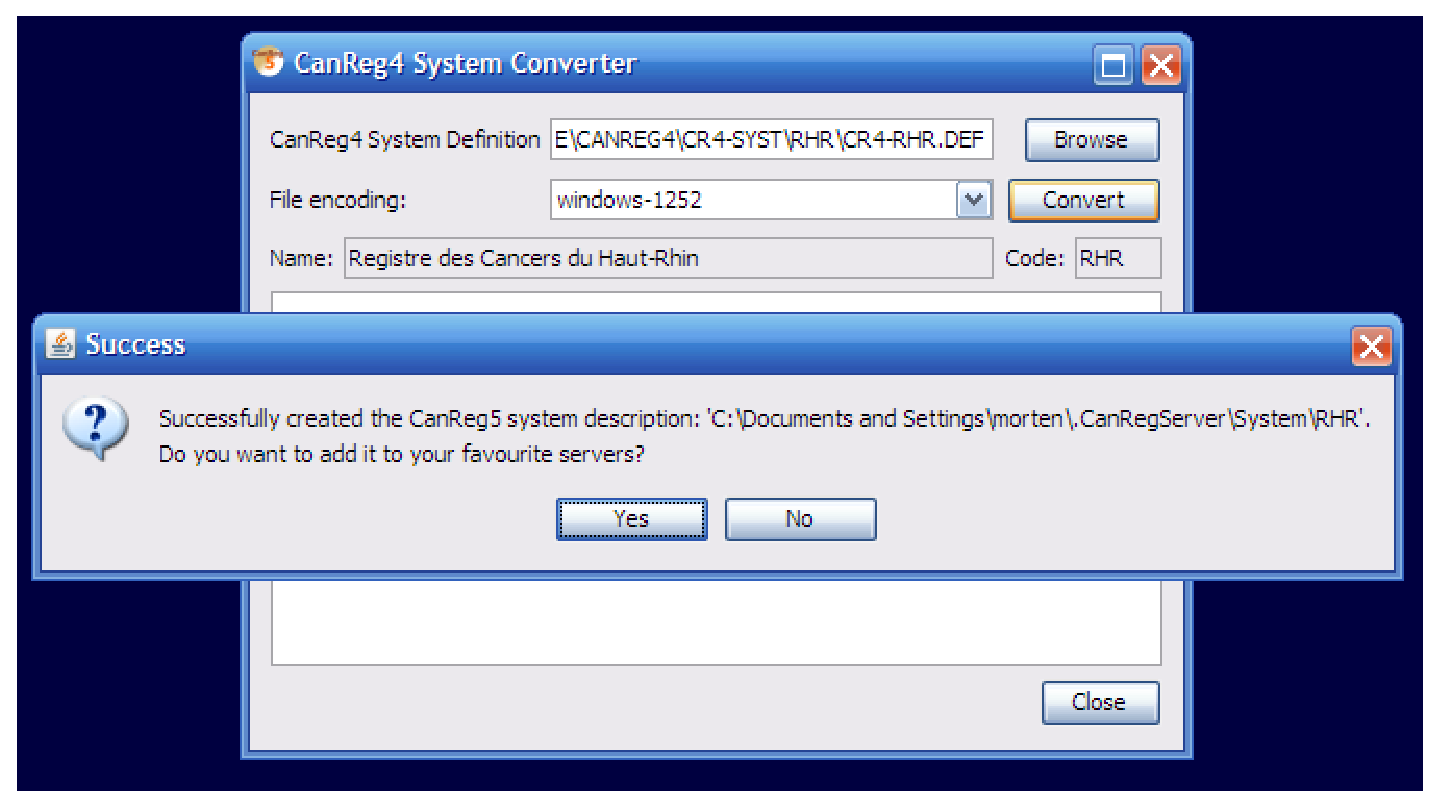
\includegraphics[width=5.4785in,height=3.1764in]{5}
\par\end{center}

\begin{flushleft}
The next step is the trickiest one during the conversion. Since we
go from a tumour based database structure with only one big table
with all the tumour and patient related information to a structure
with both a table for tumour related information and patient related
information we need to specify what variable goes in what table of
CanReg5. We recommend putting the unique patient related information
(name, date of birth and follow-up variables) in the patient table,
source information in the source table and pretty much the rest (tumour
information, age, address etc) in the tumour table.
\par\end{flushleft}

\begin{center}
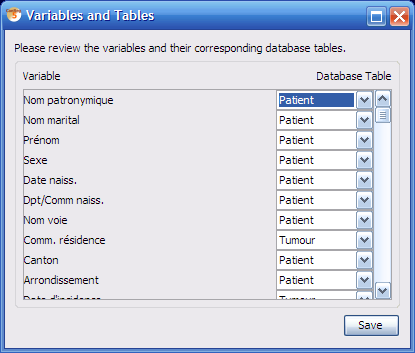
\includegraphics[width=4.32292in,height=3.67708in]{6}
\par\end{center}

\begin{flushleft}
The program presents an initial proposal that you might agree with,
but please go through one by one the variables and decide. 
\par\end{flushleft}

\begin{flushleft}
Click ``Save''. You have now created an XML\index{XML} file that
describes your CanReg5 system. 
\par\end{flushleft}

\begin{flushleft}
{\footnotesize{}Optional: Before you proceed to the next step and
launch the server you can, if you want(!), manually edit this XML
file you have created by opening it in a text editor or a dedicated
XML editor. The file is located in your user folder under .CanRegServer.
(On my machine, for example, running Windows XP it is under: C:\textbackslash{}Documents
and Settings\textbackslash{}morten\textbackslash{}.CanRegServer\textbackslash{}System.)} 
\par\end{flushleft}


\section{Setting up or modifying a CanReg system\index{modifying a CanReg system}\index{setting up a CanReg system}
using the built in editor\label{sub:Setting-up-or-modifying}}

\begin{flushleft}
To modify an existing CanReg system or set up a new one you can use
tools built into CanReg5. 
\par\end{flushleft}

\begin{center}
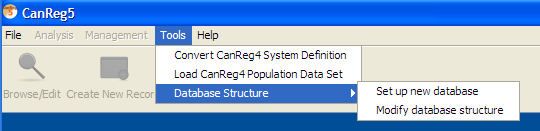
\includegraphics[width=5.4785in,height=1.3639in]{7}
\par\end{center}

\begin{flushleft}
They can be found under Tools -$>$ Database Structure. 
\par\end{flushleft}

\begin{center}
\textbf{Note: Before using this tool it is highly recommended to perform
a backup of your CanReg5 database!} 
\par\end{center}

\begin{flushleft}
For now please use ``Set up new database''. This will give you the
Modify Database Structure window. 
\par\end{flushleft}

\begin{center}
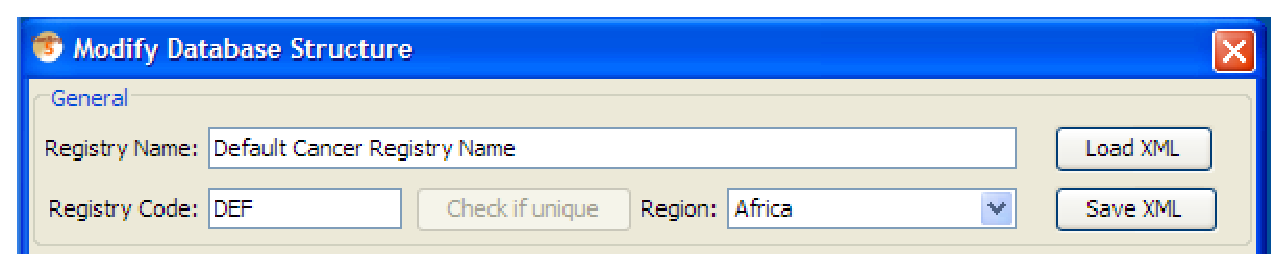
\includegraphics[width=5.4785in,height=1.0903in]{8}
\par\end{center}

\begin{flushleft}
Please click Load XML\index{XML} and either pick your own XML or,
if you start from scratch, the TRN.xml or DEF.xml found in the CanReg
installation. (You will need to load an existing XML to be able to
create a working XML for your CanReg system.) 
\par\end{flushleft}

\begin{flushleft}
Please note that certain modifications done using this tool will impact
the structure of the CanReg database to such an extent that it will
have to be rebuilt afterwards. Others like renaming groups, changing
the displayed name of a variable or reordering the variables are purely
cosmetic and do not impact the database structure as such. If you
wish to do changes to the structure of the database you'll need to
export your data prior to those changes, delete the database files
of the CanReg system, do required modifications using this tool or
directly in the XML, relaunching the CanReg server and then import
the data (this again will potentially have to be adapted to the structural
changes). CanReg will warn you if you have done changes that require
a rebuild of the database. (Fields with pink background in this editor
- as well as adding or removing variables, leads to this.)
\par\end{flushleft}

\begin{flushleft}
When this has loaded you'll see all the info specifying this CanReg
system. On the top you can specify the registry name, registry code\index{registry code}
and region of the registry. Below you have a list of the Dictionaries\index{dictionary},
then the Group\index{group}s and then the Variable\index{variable}s. 
\par\end{flushleft}

\begin{center}
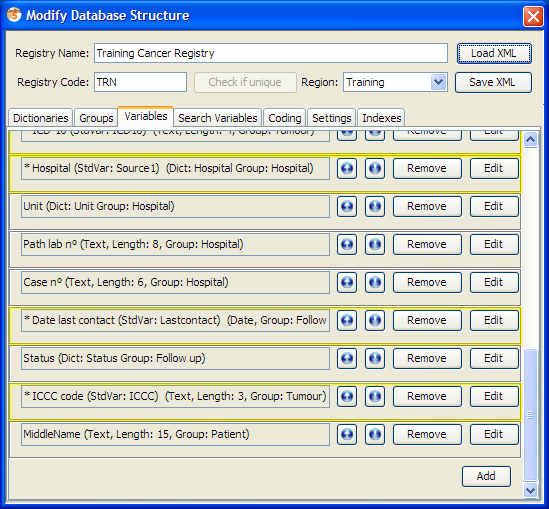
\includegraphics{modify-database-structure}
\par\end{center}

\begin{flushleft}
To add a dictionary, group or variable, click add in the proper pane.
This will then appear as the last item in the corresponding list for
you to edit. 
\par\end{flushleft}

\begin{flushleft}
Clicking edit on any button related to a dictionary, group or variable
brings up the respective editor. 
\par\end{flushleft}


\subsection{Modifying a dictionary\index{dictionary} }

\begin{center}
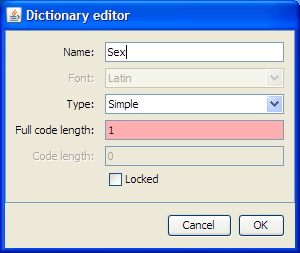
\includegraphics{dictionary-editor-sex}
\par\end{center}

\begin{flushleft}
Using the dictionary editor\index{dictionary editor} you can modify
any dictionary in CanReg5. The fields are as follows: 
\par\end{flushleft}

\begin{flushleft}
\textbf{Name:} The name of the dictionary 
\par\end{flushleft}

\begin{flushleft}
\textbf{Type:} This can either be ``Simple'' or ``Compound''.
A ``Simple'' dictionary is a plain list of codes and corresponding
labels, whereas a ``compound'' dictionary as two levels of refinement.
For example the user can pick the two first digits and then the last
digit, as in the above example. 
\par\end{flushleft}

\begin{flushleft}
\textbf{Full code length:} The number of character the codes for this
dictionary takes up in the database. 
\par\end{flushleft}

\begin{flushleft}
\textbf{Code length:} The number of characters in the first level
of refinement in the case of a compound dictionary. 
\par\end{flushleft}

\begin{flushleft}
\textbf{Locked:} Will you allow the super user to modify this dictionary
using the tools in CanReg, or should it be locked? 
\par\end{flushleft}


\subsection{Modifying a group\index{group} }

\begin{center}
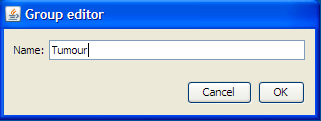
\includegraphics[width=3.34375in,height=1.26042in]{11}
\par\end{center}

\begin{flushleft}
Using the group editor\index{group editor} you can modify any group
in CanReg5. 
\par\end{flushleft}

\begin{flushleft}
\textbf{Name:} The name of the group 
\par\end{flushleft}


\subsection{Modifying a variable\index{variable} }

\begin{center}
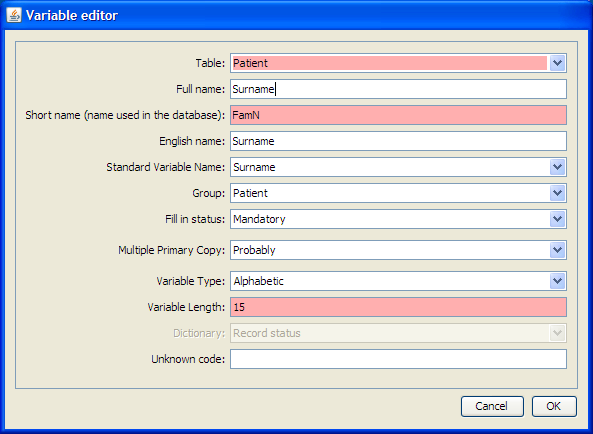
\includegraphics[width=1\columnwidth]{variable-editor-surname}
\par\end{center}

\begin{flushleft}
Using the variable editor\index{variable editor} you can modify any
variable stored in the CanReg5 database. The fields are as follows: 
\par\end{flushleft}

\begin{flushleft}
\textbf{Full name:} The name of the variable as displayed in data
entry forms etc. 
\par\end{flushleft}

\begin{flushleft}
\textbf{Short name:} The name of the variable in the database. (This
should be without any blanks and other special characters and reasonably
short.) 
\par\end{flushleft}

\begin{flushleft}
\textbf{English name:} It is useful to provide an English name for
the variable in case you want to collaborate with people in other
countries. 
\par\end{flushleft}

\begin{flushleft}
\textbf{Standard Variable Name:} This maps the variable to a standard
CanReg5 variable for the purpose of edit checks and analysis. 
\par\end{flushleft}

\begin{flushleft}
\textbf{Group:} The choice of group only affects the display during
data entry. 
\par\end{flushleft}

\begin{flushleft}
\textbf{Fill in status:} Can be set to ``Mandatory'', ``Optional'',
``Automatic'' or ``System'', depending on if you want to force
the registrar to provide this information before confirming the record. 
\par\end{flushleft}

\begin{flushleft}
\textbf{Multiple Primary Copy:} Legacy information. Leave as ``Other''. 
\par\end{flushleft}

\begin{flushleft}
\textbf{Variable Type:} Can be ``Alphabetic'' (for plain text),
``Asian text'' (legacy field, same as ``Alphabetic''), ``Date'',
``Dictionary'', ``Number'' and ``Text Area''. 
\par\end{flushleft}

\begin{flushleft}
\textbf{Variable Length:} The length of the variable in characters. 
\par\end{flushleft}

\begin{flushleft}
\textbf{Dictionary:} If you chose ``Dictionary'' as type of variable
you'll have to choose a dictionary\index{dictionary} here. 
\par\end{flushleft}

\begin{flushleft}
\textbf{Unknown code:} Here you can specify the unknown code of this
variable. 
\par\end{flushleft}

\begin{flushleft}
\textbf{Table:} Choose the table where this variable should be stored. 
\par\end{flushleft}


\subsection{Set up person search variables }

\begin{center}
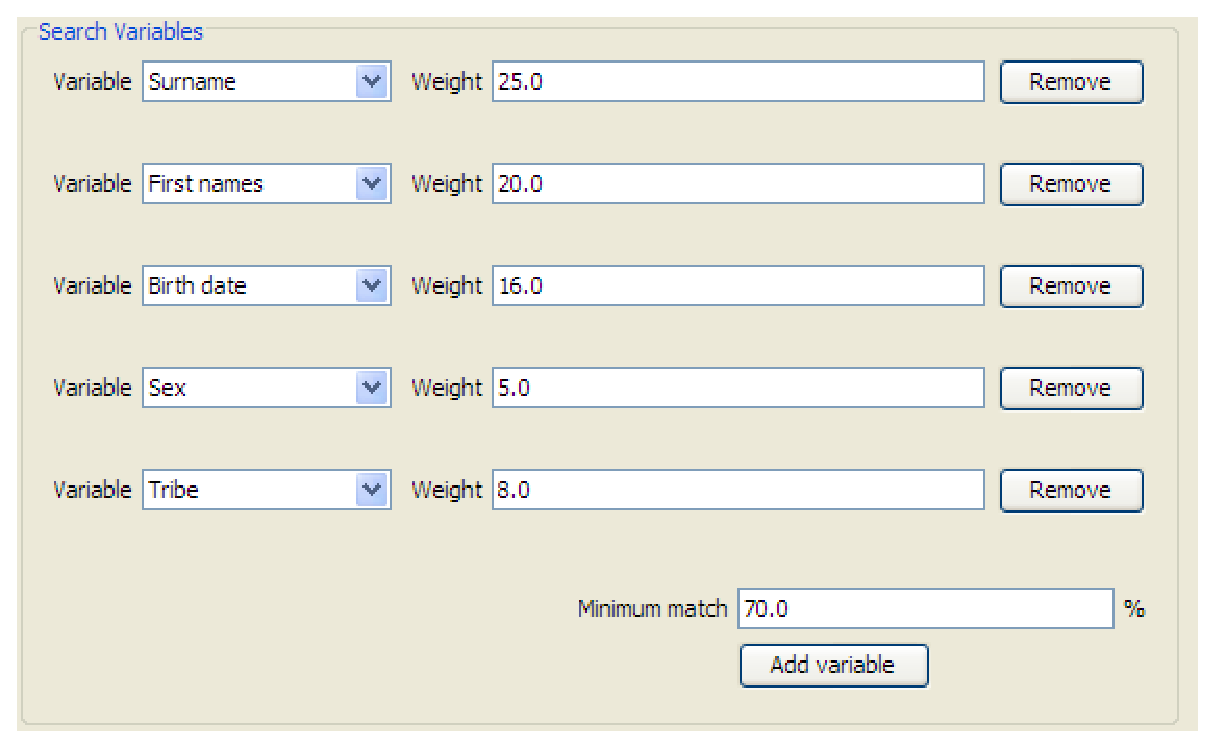
\includegraphics[width=5.4785in,height=3.4868in]{13}
\par\end{center}

\begin{flushleft}
Using this editor you can change the variables that come into play
during person search\index{person search} in CanReg5, and their respective
weights\index{weights} and minimum match\index{minimum match} criteria. 
\par\end{flushleft}


\subsection{Coding }

\begin{center}
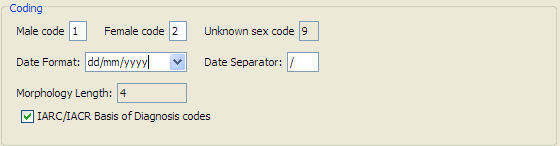
\includegraphics[width=5.4785in,height=1.5014in]{14}
\par\end{center}

\begin{flushleft}
Here you can change some coding\index{coding} settings of your CanReg
system. (Not yet implemented.) 
\par\end{flushleft}


\subsection{Settings }

\begin{center}
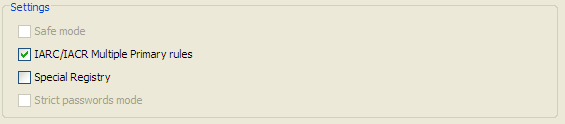
\includegraphics[width=5.4785in,height=1.2653in]{15}
\par\end{center}

\begin{flushleft}
Here you can change some settings\index{settings} of your CanReg
system. (Not yet implemented.) 
\par\end{flushleft}


\subsection{Saving the system }

\begin{flushleft}
By clicking Save XML\index{XML} the system XML will be saved to the
system folder of CanReg under the name $<$your system code$>$.xml
(for example TRN.xml), ready for use. 
\par\end{flushleft}


\section{Launching the CanReg server\index{server}}

\begin{flushleft}
After clicking ``Login'' on the welcome screen of CanReg you get
the login screen. To launch the CanReg server\index{launch the CanReg server}
click ``Settings''. Click ``Launch Server''. 
\par\end{flushleft}

\begin{center}
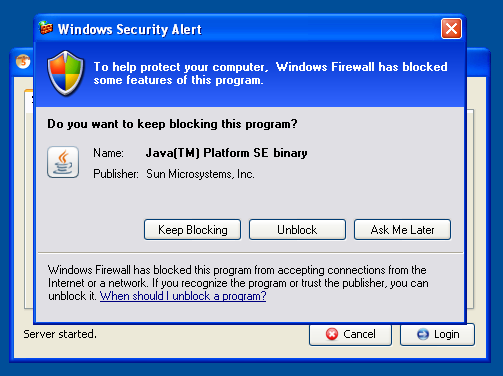
\includegraphics[width=5.23958in,height=3.91667in]{16} 
\par\end{center}

\begin{flushleft}
If you get a java firewall\index{firewall} query, please confirm
that it is OK that java can comunicate through you firewall by clicking
``Unblock'', ``OK'' or ``Yes''. If this is the first time you
launch the server on this machine it will automatically create the
database needed for CanReg5. 
\par\end{flushleft}

If your database is encrypted you will get a message regarding this
and you need to provide the database password to open it. Please note
that this can be different from your user's password.

When the CanReg5 server is running on your machine you should see
an icon in your notification area\index{notification area}.

\begin{center}
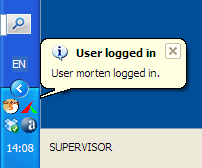
\includegraphics{notificationarea}
\par\end{center}


\section{Login\index{login@\textsf{\textbf{login}}}\label{sub:Login}}

\begin{flushleft}
After launching the server you can log on to your CanReg system. 
\par\end{flushleft}


\subsection{Locally }

\begin{flushleft}
If you want to log in to a CanReg server running on your local machine\index{local machine},
after either installing a CanReg5 system XML or converted your CanReg4
system definition files you go to the ``System'' tab of the ``Login''-window
and choose your server from the drop down list. (Most probably already
selected.) (The default username is ``morten'' and password is ``ervik''.
(All in small letters with no double quotes.) Click ``Login'' and
you'll be logged on.) 
\par\end{flushleft}

\begin{flushleft}
If you get an error message saying ``Could not log in to the CanReg
server on localhost with the given credentials.'', please make sure
that you have entered the correct username and password and that the
server is indeed running. (See ``Launching the CanReg server'' above.) 
\par\end{flushleft}

\begin{center}
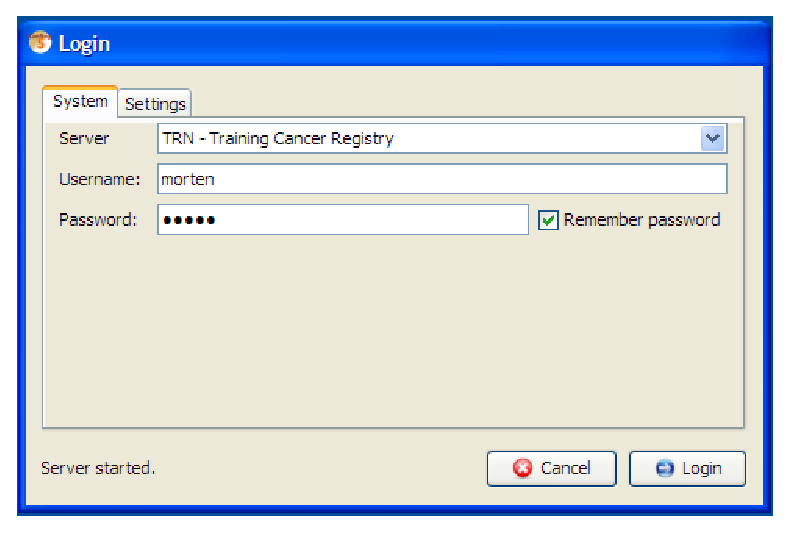
\includegraphics{CanRegLoginScreen}
\par\end{center}


\subsection{In a network }

\begin{flushleft}
If you want to log on to a CanReg server running on another machine
in your network\index{network} you need to know the address of that
machine. (Either it's IP address\index{IP address} or name on the
network\index{name on the network}.) 
\par\end{flushleft}

\begin{flushleft}
To find the IP address of a CanReg server you can go to the Settings
tab on the ``Login''-window and tick ``Advanced'' to get access
to some more advanced tools, like the ``Get IP Address'' tool. Click
this and you will get a message saying ``The IP address of (your
machine) is www.xxx.yyy.zzz. (Most probably something like 10.0.0.x
or 192.168.0.x.) Take a note of those numbers. 
\par\end{flushleft}

\begin{flushleft}
Launch CanReg on the machine you want to run CanReg on. Click ``Login''
to get to the ``Login'' screen. There you can click ``Settings''
and type the IP address, www.xxx.yyy.zzz, you found above in the ``Server
URL'' field along with the system code for your registry. (For example
TRN.) If you click ``Add server to list'' the program will test
the connection to the server and if this is OK this network server
will be added to the list of servers you can log in to from this CanReg
installation. 
\par\end{flushleft}

\begin{flushleft}
Click the ``System'' tab and choose this networked server from the
drop down list of servers, enter username and password. (The default
username is ``morten'' and password is ``ervik''. (All in small
letters with no double quotes.) Click ``Login'' and you'll be logged
on.) Click ``Login'' and you'll be logged on.) 
\par\end{flushleft}

\begin{flushleft}
If you get an error message saying ``Could not log in to the CanReg
server on localhost with the given credentials.'', please make sure
that you have entered the correct username and password and that the
server is indeed running. (See ``Launching the CanReg server'' above.) 
\par\end{flushleft}

\begin{flushleft}
The next time you want to log on to this server all you have to do
is launch CanReg, select this server, enter username and password
and click ``Login''. 
\par\end{flushleft}

\begin{flushleft}
Please note that you do \emph{not} need to install the system definition
or convert from CanReg4. You only need the code (for example TRN)
of the CanReg system you want to connect to.
\par\end{flushleft}


\section{Import the dictionaries\index{import dictionaries}}

\begin{flushleft}
If you are migrating from CanReg4 make sure to export the most updated
dictionary from your CanReg4 system. (In CanReg4: ``Data Entry'',
``Dictionary'', ``Export dictionary to text file'') If you want
to use the demo system, the dictionary is located in: demo/dictionary. 
\par\end{flushleft}
\begin{itemize}
\item \begin{flushleft}
Go to ``File'', ``Data Entry'', ``Edit dictionary'' in CanReg5
\par\end{flushleft}
\end{itemize}
\begin{center}
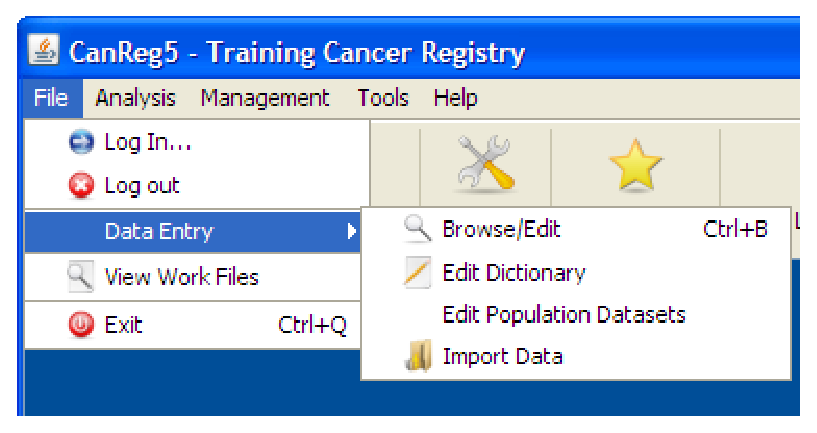
\includegraphics[width=3.91667in,height=2in]{17}
\par\end{center}
\begin{itemize}
\item \begin{flushleft}
Click on ``Import complete dictionary from file''.
\par\end{flushleft}
\end{itemize}
\begin{center}
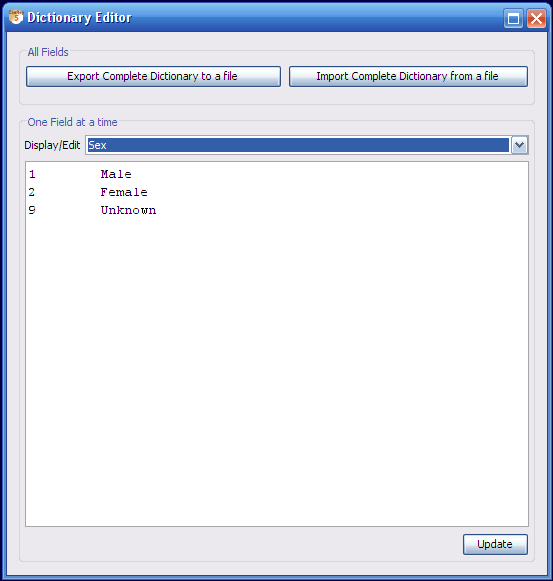
\includegraphics[width=4.79792in,height=5.04097in]{18}
\par\end{center}
\begin{itemize}
\item \begin{flushleft}
Browse and select the dictionary from you CanReg4 work folder or elsewhere. 
\par\end{flushleft}
\item \begin{flushleft}
Do Preview 
\par\end{flushleft}
\item \begin{flushleft}
Tick ``CanReg4 Format'' if you are migrating from CanReg4, leave
unticked if you are using the demo system or otherwise are importing
a CanReg5 formatted dictionary.
\par\end{flushleft}
\end{itemize}
\begin{center}
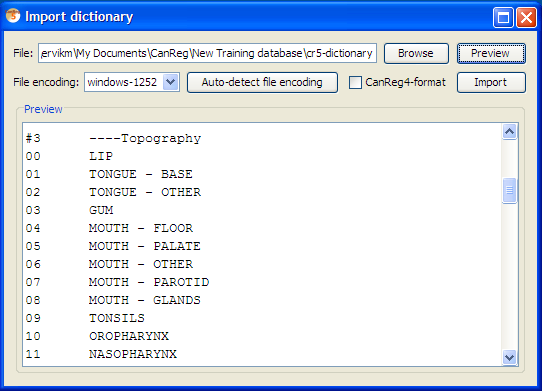
\includegraphics{dictionaryimport}
\par\end{center}
\begin{itemize}
\item \begin{flushleft}
Click Import. This might take some time. Please note the bar in the
lower right indicating that the program is busy. 
\par\end{flushleft}
\item \begin{flushleft}
Afterwards you will receive a message of success imported. 
\par\end{flushleft}
\item \begin{flushleft}
Click OK. 
\par\end{flushleft}
\item \begin{flushleft}
Go back to ``File'', ``Data Entry'', ``Edit dictionary'' and
verify that the dictionaries have been imported. 
\par\end{flushleft}
\end{itemize}

\section{Import the data\index{import data from CanReg4} from CanReg4\label{sub:Import-the-data}}

\begin{flushleft}
Make sure to export the most updated data from your \index{CanReg4}CanReg4
system. 
\par\end{flushleft}
\begin{itemize}
\item \begin{flushleft}
In CanReg4: ``Analysis'', ``Export data'' 
\par\end{flushleft}
\item \begin{flushleft}
Tick ``Export all variables''. 
\par\end{flushleft}
\item \begin{flushleft}
Choose variables names short 
\par\end{flushleft}
\item \begin{flushleft}
\textbf{Under ``Export File options'' choose ``Comma separated
variables''} 
\par\end{flushleft}
\item \begin{flushleft}
Untick ``Format date'' 
\par\end{flushleft}
\item \begin{flushleft}
Untick ``Correct Unknown'' 
\par\end{flushleft}
\item \begin{flushleft}
Click ``write data to file'' and pick a file name that you can find
back easily in CanReg5. For example on the desktop. Click ``save''. 
\par\end{flushleft}
\item \begin{flushleft}
Take a look at the data you have now exported and close CanReg4. 
\par\end{flushleft}
\item \begin{flushleft}
Back in CanReg5 do ``File'', ``Data Entry'' and ``Import Data''.
\par\end{flushleft}
\end{itemize}
\begin{center}
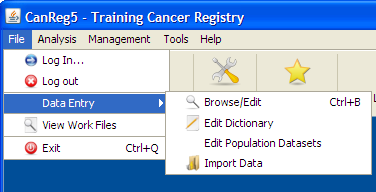
\includegraphics[width=3.91667in,height=2in]{20}
\par\end{center}
\begin{itemize}
\item \begin{flushleft}
The program will ask you if you have all your data in one file. Answer
``yes'' as this is the case when migrating from CanReg4. 
\par\end{flushleft}
\item \begin{flushleft}
Click ``Browse'' and locate the file from step A. Select it and
click ``Open''. You can if you want preview the file to see that
you picked the right one and that the file looks OK. If for example
Arabic names are garbled you should try to choose another ``File
encoding\index{file encoding}'' (Default for Arabic text is ISO-8859-6). 
\par\end{flushleft}
\item \begin{flushleft}
\textbf{Set ``Separating character\index{separating character@separating\textbf{ }character}''
to Comma.} (Or whatever separating characters your file has.)
\par\end{flushleft}
\end{itemize}
\begin{center}
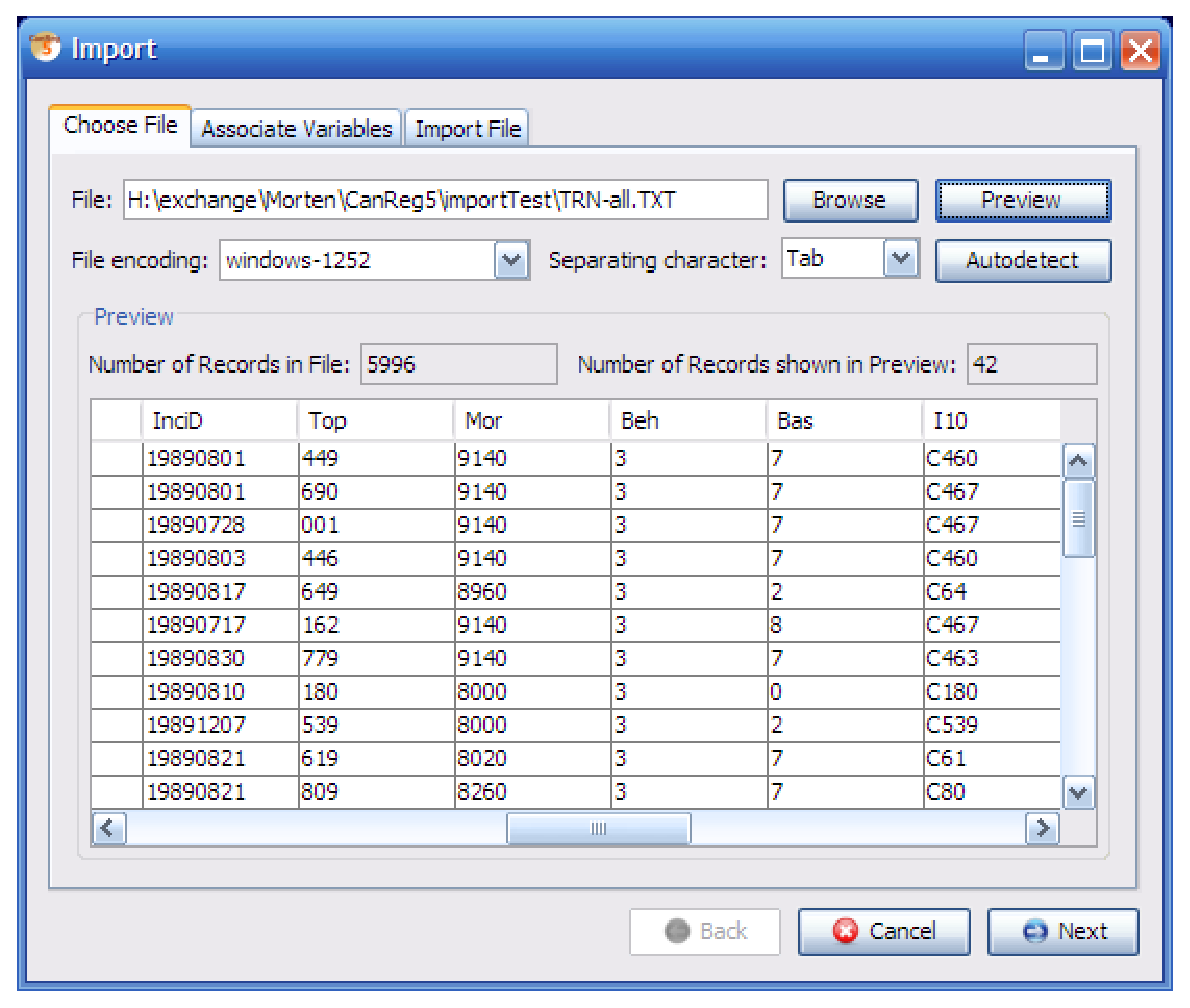
\includegraphics[width=5.00069in,height=4.21667in]{21}
\par\end{center}
\begin{itemize}
\item \begin{flushleft}
Click Preview to see that the data looks OK. 
\par\end{flushleft}
\item \begin{flushleft}
Click ``Next'' (or select the tab ``Associate Variables'') 
\par\end{flushleft}
\item \begin{flushleft}
This lets you associate the variables in the file to import with the
variables in the database. CanReg5 will find most of these associations
by itself, but you should revise them to see if they look OK. Look
for variable names in bold, as they are the one that are not assigned
at all. 
\par\end{flushleft}
\item \begin{flushleft}
Click ``Next'' (or select the tab ``Import File'') 
\par\end{flushleft}
\item \begin{flushleft}
Click ``Import'' (leave everything as by default -- the import function
only works on empty CanReg databases as per now\ldots{}) 
\par\end{flushleft}
\item \begin{flushleft}
Let CanReg5 import the data (this might take a while) and click ``OK''. 
\par\end{flushleft}
\item \begin{flushleft}
Click ``Browse/Edit'' and ``Refresh Table'' to see that the data
has arrived well. 
\par\end{flushleft}
\end{itemize}

\section{Import data from other programs\index{import data from other programs}}

\begin{flushleft}
You can import data from other programs than CanReg4 by using the
import tool in CanReg5. The only thing to pay attention to is that
the data has to be coded in exactly the same way as in the CanReg5
database. 
\par\end{flushleft}
\begin{itemize}
\item \begin{flushleft}
Dates should be coded as year month day (yyyyMMdd) -- ISO 8601
\par\end{flushleft}
\item \begin{flushleft}
Topography in 3 digits ICD-O-3 with no leading C. 
\par\end{flushleft}
\item \begin{flushleft}
Morphology in 4 (or 5) digits ICD-O-3.
\par\end{flushleft}
\end{itemize}
\begin{flushleft}
Other fields with dictionaries, like for example addresses should
follow the dictionary defined for them in CanReg5. 
\par\end{flushleft}

\begin{flushleft}
The data can either be in a single file as the example for CanReg4,
or in one separate file for patient-information, tumour information
and source information (with pointers to link sources to tumours and
tumours to patients). 
\par\end{flushleft}

\newpage{}


\part{Working with CanReg5}


\chapter{Start}


\section{Welcome screen}

\begin{flushleft}
There are two options in this CanReg5 welcome screen\index{welcome screen}:
\textquotedbl{}Login to CanReg\textquotedbl{} and \textquotedbl{}Install
New System\textquotedbl{}.
\par\end{flushleft}

\begin{center}
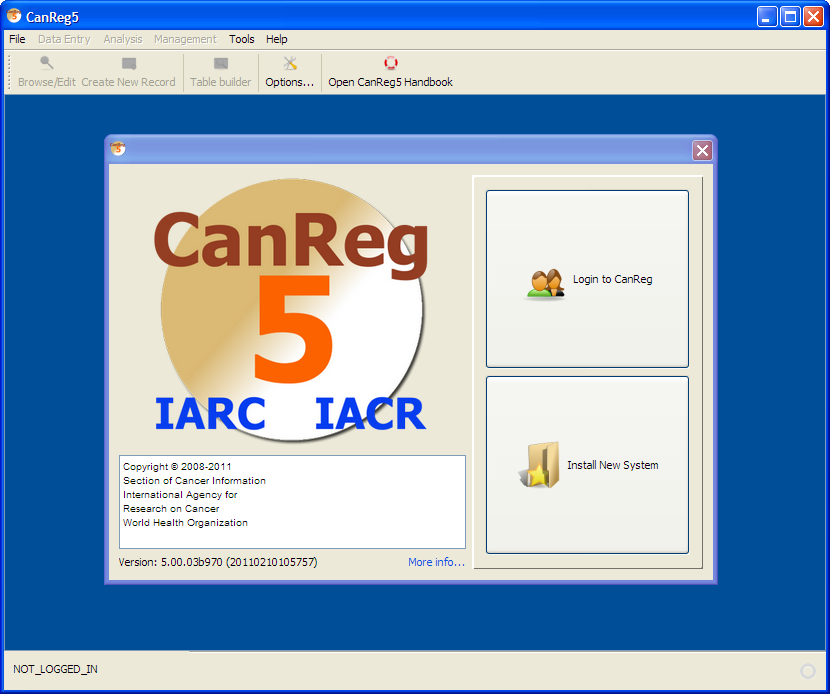
\includegraphics[scale=0.5]{CanRegWelcomeScreen}
\par\end{center}


\section{Login to CanReg}

If CanReg5 has already been setup on this computer for your cancer
registry, then click on this option to pass to the \textquotedbl{}Login/Password\textquotedbl{}
panel. (See \vref{sub:Login} for more information.)


\subsection{Advanced login settings}

\begin{figure}
\begin{centering}
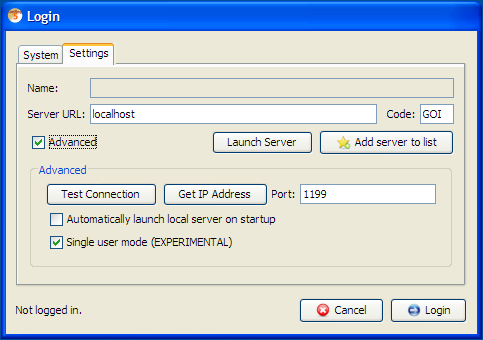
\includegraphics{loginsettings}
\par\end{centering}

\protect\caption{\label{fig:Login-settings}Login settings}


\end{figure}


Under Settings you can tick Advanced to get access to some more advanced
settings for CanReg. (See figure \vref{fig:Login-settings}.)


\subsubsection{Test connection }

will test the connection to the server specified - without connecting
to it.


\subsubsection{Get IP Address}

will try to get the ip address of the URL specified in the Server
URL field. If this is set to localhost it will give you the IP address
of the machine you are on. This can be usefull when installing CanReg
in a network.


\subsubsection{Port}

lets you change the port the server is running on. This can be useful
if another program is running on the default port and you want to
change that or if you need to tunnel CanReg traffic through a VPN-network
or similar.


\subsubsection{Automatically launch local server on startup}

is by default ticked after installing a new XML. This does what it
says - it will try to launch the last used CanReg server on this machine
when starting CanReg. Basically it clicks ``Launch Server'' for
you when opening the login screen.


\subsubsection{Single user mode}

lets you log on to your CanReg system without starting the network
components. This can be useful if you are the only user on CanReg
this session. Like this you avoid network related errors due to for
example laptops falling asleep. Also, it is slightly safer, since
you can be sure that nobody can log on to your system but you (even
if they have gotten hold of your username and password and server
address).


\section{Install New System}

The CanReg5 program has been installed but you wish to add the Registry
definition for a particular Cancer Registry. To install a new system
you can use this module. Click browse and choose the XML-file that
corresponds to your system. (See \vref{sub:Install-a-new} for more
information.)\newpage{}


\chapter{\index{data entry}Data entry}

From the data entry menu you can open the Browse/edit data view, edit
dictionary view, edit population datasets view or import data view.


\section{Browse/edit}

This part of CanReg5 allows you to view and edit the database records.

For Data Entry purposes, you can use this Browse part to look for
a particular record to Edit, or to see if a particular person has
a cancer notification already stored.

The table below shows the data - move (with the \textquotedbl{}Scroll
Bars\textquotedbl{}) horizontally to see other variables, or vertically
to view other records.

You can use the Filter, Index and Ranges to select which records to
show, and the Variables radio buttons to select the variables columns.

Use these buttons to go to the Edit Form:

- Create next record: If you have checked that the patient has no
record already, use this option to create a new blank edit form. The
next available registration number will be assigned when you save
the record.

- Edit Table record: to edit the record highlighted by the blue bar
in the data table.

- Edit/create Patient ID: Before clicking this button, fill in the
Registration number of the record you wish to edit. If the record
exists already, you can edit it; if not, this number will be assigned
to a new blank record. USE THIS OPTION TO SET THE REGISTRATION NUMBER
FOR YOUR FIRST RECORD.

- Re-draw table:

If you have made changes to the database, use this button to update
the table displayed.


\subsection{Table\index{table}}

This lets you select the table to look at.


\subsection{Sorty by\index{sorty by}\label{sub:Sorty-by}}

The records will be ordered (or sorted) by the variable chosen.


\subsection{Range\index{range}\label{sub:Range}}

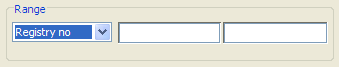
\includegraphics{range}

You can specify the Range start and end values for that sequenced
variable.

Example of how to use:
\begin{itemize}
\item Sort by Date of Incidence,
\item show records of years 2000 and 2001 only:
\item Range = Incidence Date
\item Range Start = 2000
\item Range End = 20019999
\end{itemize}

\subsection{Filter\index{filter}\label{sub:Filter}}

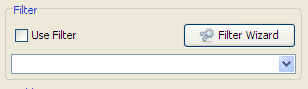
\includegraphics{filter}

To select records. (Use \textquotedbl{}Range\textquotedbl{} as primary
selection - it is quicker)

\begin{tabular}{|c|>{\centering}p{0.75\linewidth}|}
\hline 
Operator\index{operator} & Description\tabularnewline
\hline 
\hline 
= & Equal\tabularnewline
\hline 
<>  & Not equal\tabularnewline
\hline 
> & Greater than\tabularnewline
\hline 
< & Less than\tabularnewline
\hline 
>= & Greater than or equal\tabularnewline
\hline 
<= & Less than or equal\tabularnewline
\hline 
BETWEEN & Between an inclusive range\tabularnewline
\hline 
LIKE & Search for a pattern (use \% as wildcard)\tabularnewline
\hline 
IN & If you know the exact value you want to return for at least one of
the columns.\tabularnewline
\hline 
\end{tabular}

\begin{tabular}{|c|c|}
\hline 
Logical Operator\index{logical operator} & Description\tabularnewline
\hline 
\hline 
AND & match both criterias\tabularnewline
\hline 
OR & match one of the criterias\tabularnewline
\hline 
\end{tabular}


\subsubsection{Examples of how to use}
\begin{itemize}
\item sex = \textquoteright 1\textquoteright{} (all male cases.)
\item age >= 60 (cases aged 60 and more.)
\item sex = \textquoteright 2\textquoteright{} and age < 60 (female cases
aged more than 60.)
\item age BETWEEN 45 AND 60 (cases from patients aged from 45 to 60 (inclusive))
\item age <15 OR age>60 (patients aged less than 15 and more than 60)
\item name = 'Smith' (Name is \textquotedblleft Smith\textquotedblright )
\item name LIKE 'Sm\%' (Name begins with \textquotedblleft Sm\textquotedblright .)
\item basis = \textquoteright 7\textquoteright{} or Basis = \textquoteright 5\textquoteright{}
(Basis is 7 or 5.)
\item topog LIKE '50\%' (for all Breast cases.)
\end{itemize}

\subsection{Filter wizard\index{filter wizard}}

\begin{figure}
\begin{centering}
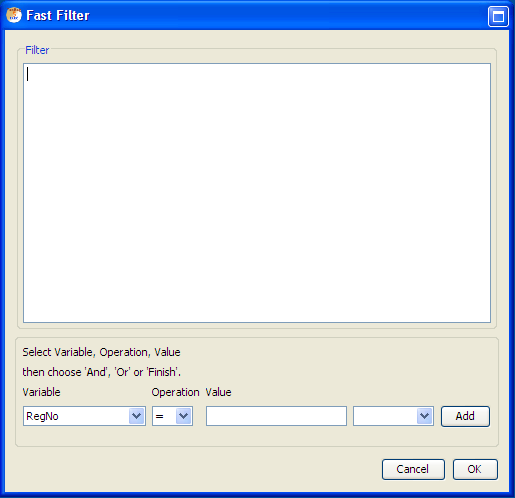
\includegraphics{filterwizard}
\par\end{centering}

\protect\caption{\label{fig:Filter-Wizard}Filter Wizard}
\end{figure}


The filter wizard is here to help you build filters. (See figure \vref{fig:Filter-Wizard}.)
It is a fast method to specify filter, or selection, criteria.


\subsubsection{For example}

, to select

Females over 60 years old.... (make sure you have selected Tumour+Patient
table)

Launch Filter Wizard and click on ...
\begin{enumerate}
\item Variable - \textquotedbl{}Sex\textquotedbl{}
\item Operator - \textquotedbl{}=\textquotedbl{}
\item Value - \textquotedbl{}Female\textquotedbl{} (from Dictionary)
\item Logical Operator - \textquotedbl{}And\textquotedbl{}
\item \textquotedbl{}Add\textquotedbl{}
\item Variable - \textquotedbl{}Age\textquotedbl{}
\item Operator - \textquotedbl{}>\textquotedbl{}
\item Value - type \textquotedbl{}60\textquotedbl{}
\item \textquotedbl{}Add\textquotedbl{}
\item \textquotedbl{}OK\textquotedbl{}
\end{enumerate}
For some combinations using \textquotedbl{}AND\textquotedbl{} and
\textquotedbl{}OR\textquotedbl{} you may need to add brackets after.

e.g.

Topog = \textquoteleft 220\textquoteright{} AND (Basis=\textquoteright 1\textquoteright{}
OR Basis=\textquoteright 2\textquoteright )


\subsection{Display variables\index{display variables}}

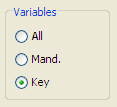
\includegraphics{displayvariables}

Click on a \textquotedbl{}radio button\textquotedbl{} above to display
either:

- All variables

- Mandatory variables (those that MUST be filled in the Edit form)

- Key variables (Names, Age, Date Incidence, Topog etc)


\subsection{Navigate buttons\index{navigate buttons}}

Click on the Navigation buttons below to move record: Top, Bottom,
Up, Down.


\section{Edit record\index{edit record}}

\begin{flushleft}
To get to a data entry form either press Create New Record\index{create new record}
from the menu bar
\par\end{flushleft}

\begin{center}

\includegraphics[width=4.11458in,height=0.697917in]{24} 
\par\end{center}

\begin{flushleft}
or enter a new record number in the browser and click ``Edit Patient
ID:''
\par\end{flushleft}

\begin{center}

\includegraphics[width=2.47917in,height=0.302083in]{25}
\par\end{center}

or double click on any record in the browser.

\begin{center}
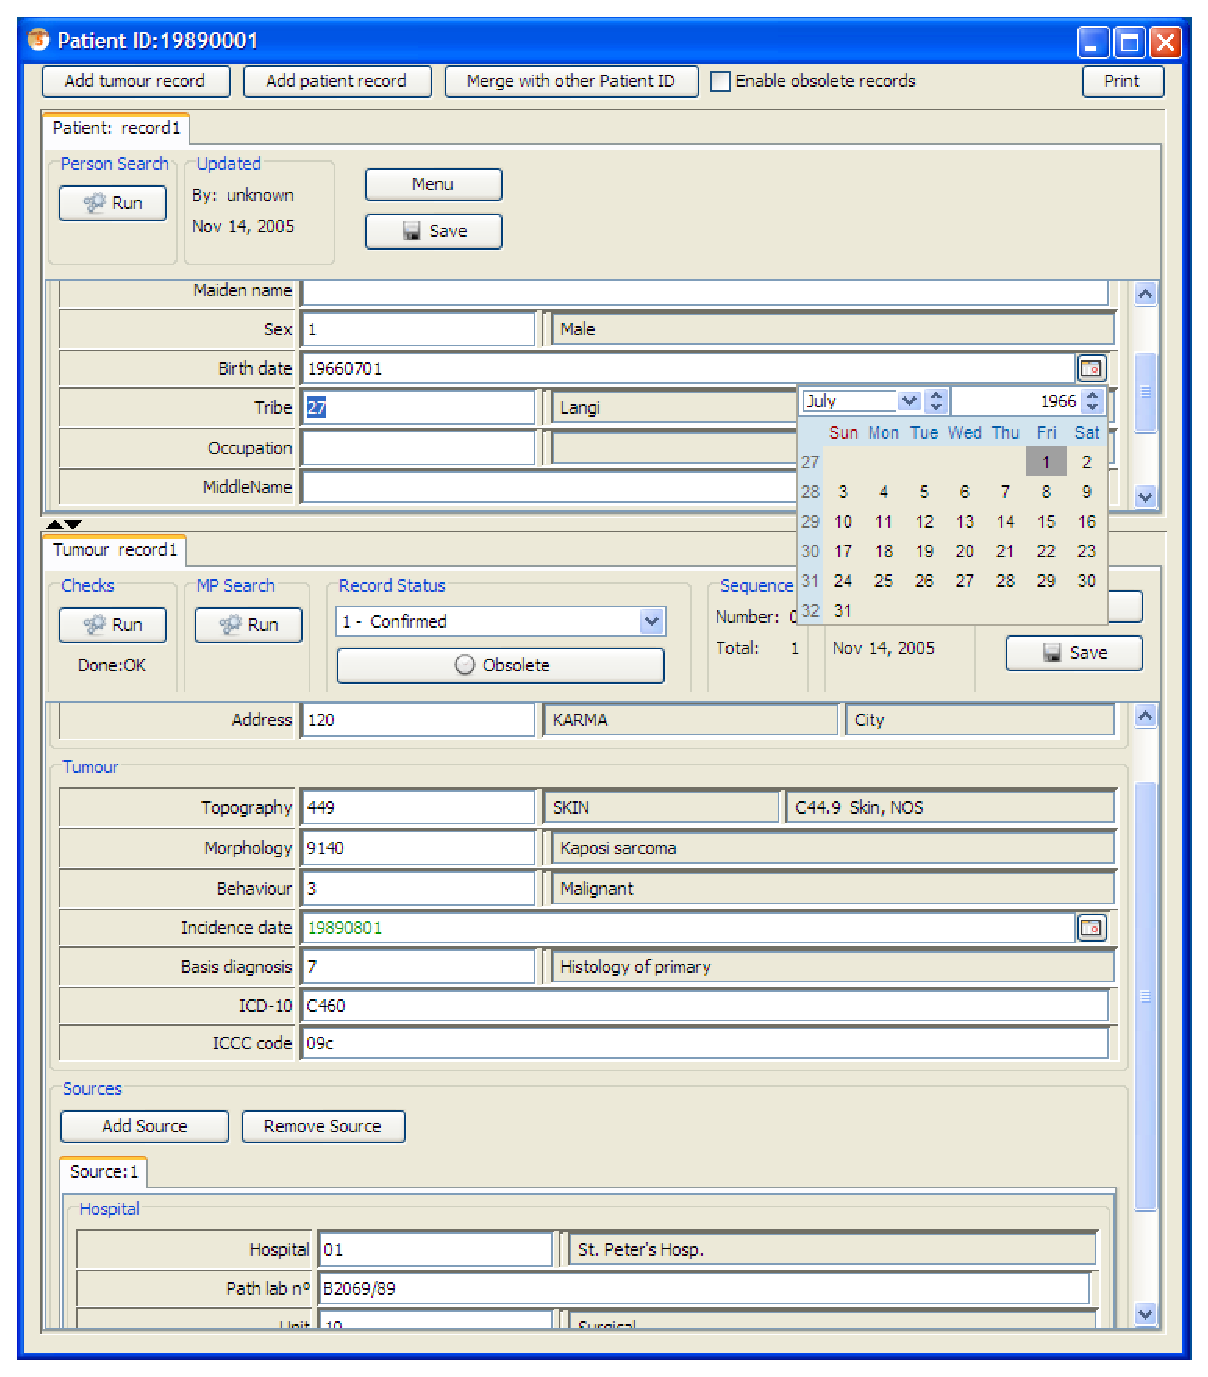
\includegraphics[scale=0.5]{DataEntryExample}
\par\end{center}

You can move around the Data Entry form in the following ways:

- Tab and shift-tab to move to the next or previous variable;

With the mouse, simply click on the variable you wish to edit, or
on the dictionary box to select from the popup of the valid dictionary
codes.

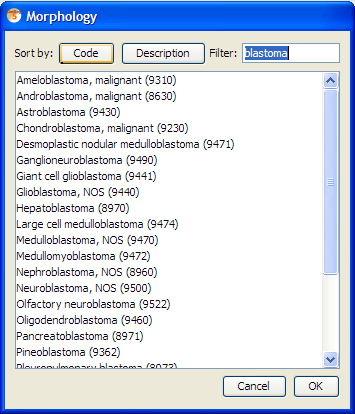
\includegraphics{dictionaryelementchooser}

\begin{flushleft}
The pink fields\index{pink fields} are the mandatory\index{mandatory variables}
ones. (Date format is still set to yyyyMMdd, but this will be improved
later.)
\par\end{flushleft}

When you have finished entering the data, you must perform the checks
as described in the system variables part below.


\subsection{System variables\index{system variables}}

After data entry, you must perform the following steps:


\paragraph{Person Search\index{person search}}

Searches for any records that might belong to the same person.


\paragraph{Check\index{check}}

Performs various consistency checks (\vref{sub:Check})on the data
you have entered.


\paragraph{Record Status\index{record Status}}

All new records are set to \textquotedbl{}Pending\textquotedbl{} and
cannot be \textquotedbl{}Confirmed\textquotedbl{} until the \textquotedbl{}Check\textquotedbl{}
and the \textquotedbl{}Person search\textquotedbl{} have been successfully
performed. Only confirmed cases are used for analysis. Only a user
with \textquotedbl{}Supervisor\textquotedbl{} permission level can
confirm rare or multiple primary cases, or delete records.


\paragraph{Save\index{save record}}

Save record to the database

The \textquotedbl{}Updated\textquotedbl{} box shows the date that
the record was last edited and by whom.


\subsection{Obsolete button. }

\begin{flushleft}
This will flag the record as obsolete\index{obsolete}, so that it
will not show up in analysis\index{analysis}. It is a way to keep
duplicate records\index{duplicate records} that might contain valuable
information.
\par\end{flushleft}


\subsection{Check\index{check}\label{sub:Check}}

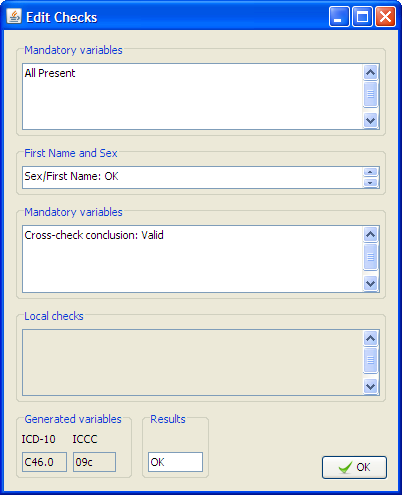
\includegraphics{check}

Any variables found in error or query will be marked in red in the
data entry form.

There are three sections to the checks:


\paragraph{Mandatory variable\index{mandatory variable}s}

Indicates any variables, defined as mandatory for your Registry, that
have not been filled in. If the value is really not available, then
fill in \textquotedbl{}9\textquotedbl{} or \textquotedbl{}99\textquotedbl{}
etc. - the code for \textquotedbl{}Unknown\textquotedbl{}.


\paragraph{First Name\index{name} and Sex\index{sex}}

Checks the combination of First Name and Sex. e.g. \textquotedbl{}Mary\textquotedbl{},
\textquotedbl{}male\textquotedbl{} would probably be an error! A name
that is really used by both sexes can be defined as \textquotedbl{}Unisex\textquotedbl{}.


\paragraph{Cross checks\index{cross checks}\index{checks}}

These are the same consistency checks as in the IARC Tools \textquotedbl{}Check\textquotedbl{}
program. Some combinations would be marked as errors:

e.g. Sex = Female and Topography = Prostate, while others could be
marked as \textquotedbl{}Rare\textquotedbl{}. Only a Supervisor can
confirm a Rare case.

As well as performing these checks, this function also determines
the ICD-10 code derived from the ICD-O Topography and Morphology.

For more information on these checks please see: http://www.iacr.com.fr/TechRep42-MPrules.pdf

(The following checks are implemented in CanReg5: \textquotedbl{}Age
and Morphology\textquotedbl{}, \textquotedbl{}Age and Topography\textquotedbl{},
\textquotedbl{}Age, IncidenceDate, and BirthDate\textquotedbl{}, \textquotedbl{}Age,
Topography, and Morphology\textquotedbl{}, \textquotedbl{}Basis\textquotedbl{},
\textquotedbl{}DateOfLastContact\textquotedbl{}, \textquotedbl{}Grade\textquotedbl{},
\textquotedbl{}Morphology\textquotedbl{}, \textquotedbl{}Sex and Morphology\textquotedbl{},
\textquotedbl{}Sex and Topography\textquotedbl{}, \textquotedbl{}Topography
and Behaviour\textquotedbl{}, \textquotedbl{}Topography and Morphology\textquotedbl{},
and \textquotedbl{}Topography\textquotedbl{}.)


\subsection{Person search\index{person search}}

The whole database is searched using probability matching for any
records that might belong to the same person. All personal data such
as Date of Birth, Place of Residence, Id Number, plus a phonetically
simplified form of the name are used in this search. (This can be
tailored by the administrator of the CanReg5 system.) Any other record
with a percentage match higher than the \textquotedbl{}Minimum Match\textquotedbl{}
is displayed.

If no match is found, a message will be displayed to that effect.

Otherwise, the computer only displays possibilities - YOU must decide
if it really is the same person.


\section{Dictionary editor\index{dictionary editor}}

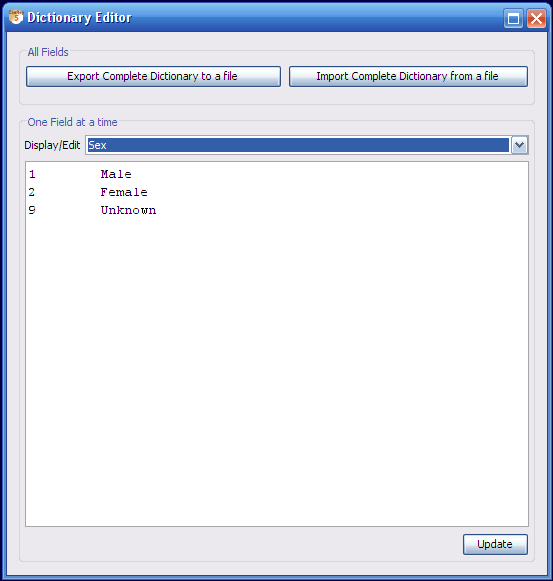
\includegraphics[width=1\columnwidth]{dictionaryeditor}

The dictionary editor lets the supervisor users edit the coding schemes
of the various variables in CanReg5.


\subsection{Export Dictionary\index{export dictionary} to file}

Export the current set of CanReg5 dictionaries to a tab-separated
file for editing in for example Excel.


\subsection{Display/edit \dots{} Select}

This will display any dictionary picked by the user for editing directly
in CanReg. The format will be standard tab-separated values so that
the user can also copy and paste this into general spreadsheet applications.


\subsection{Update}

This will import the dictionary picked by the user from the text area.
The format must be tab-separated values. This means that the users
can copy and paste directly form general spreadsheet applications
(i.e. Excel).


\subsection{Import Dictionary\index{import dictionary} from file}

Import a complete set of CanReg5 dictionaries from a tab-separated
file. (Or a two-space-separated CanReg4 dictionary.)

\begin{center}
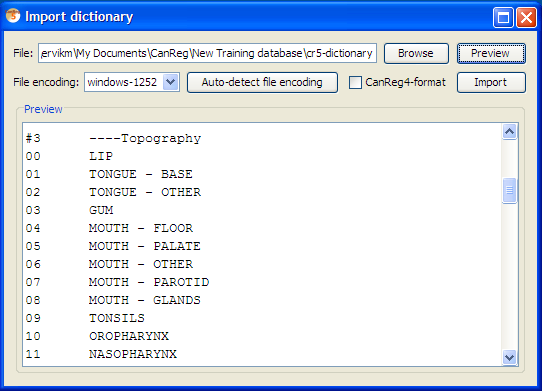
\includegraphics[width=1\columnwidth]{dictionaryimport}
\par\end{center}


\section{Population Dataset Editor}


\subsection{Manual entry/validation}

\begin{flushleft}
The Population Dataset\index{population dataset editor}\index{population dataset}
\index{PDS}editor lets you edit population data set to be used in
the table builder. This is located under File -- Data Entry Edit Population
Dataset: 
\par\end{flushleft}

\begin{center}
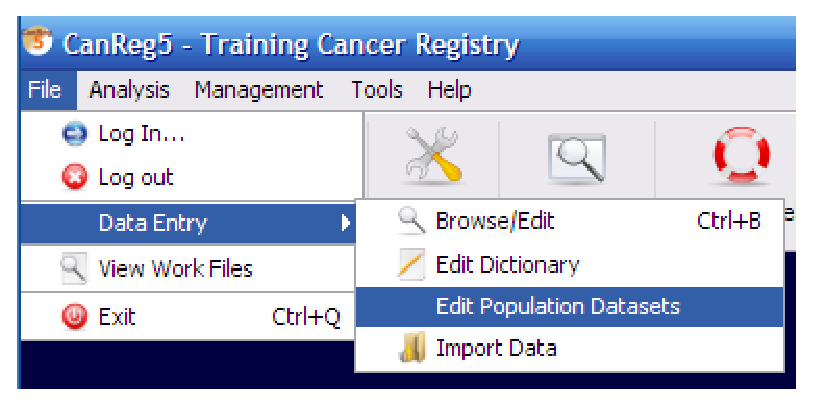
\includegraphics[width=3.89583in,height=1.86458in]{32}
\par\end{center}

\begin{flushleft}
When you start it you get to the list of all your population datasets.
\par\end{flushleft}

\begin{center}
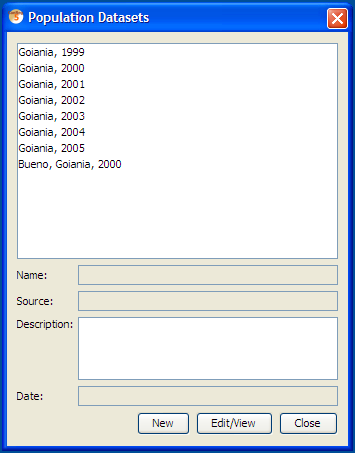
\includegraphics{popeditor1}
\par\end{center}

\begin{flushleft}
Add one by clicking New. This opens the Population Dataset editor: 
\par\end{flushleft}

\begin{center}
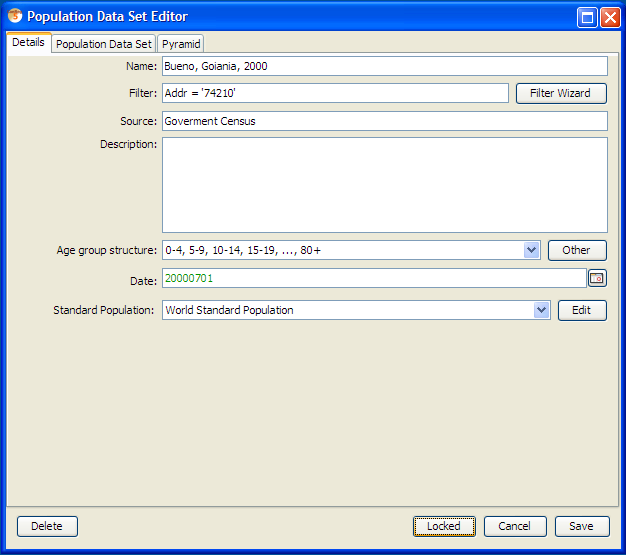
\includegraphics[width=1\columnwidth]{popeditor2}
\par\end{center}

\begin{flushleft}
Fill in the details:
\par\end{flushleft}
\begin{itemize}
\item \begin{flushleft}
A name for the dataset 
\par\end{flushleft}
\item \begin{flushleft}
\textquotedbl{}Filter\textquotedbl{} or selection criteria, so the
program only selects records corresponding to the population (e.g.
Address code >= 10 and Address code <= 19) (Basically if it does not
cover your entire area of your database.)
\par\end{flushleft}
\item \begin{flushleft}
A source of this data (e.g. whether Goverment Census, or Estimation).
\par\end{flushleft}
\item \begin{flushleft}
Some description (less than 255 characters) 
\par\end{flushleft}
\item \begin{flushleft}
Choose the age group structure\index{age group structure}. 
\par\end{flushleft}
\item \begin{flushleft}
Set the date when the population was at this amount. (In the example
above it is mid 1992) 
\par\end{flushleft}
\item \begin{flushleft}
The Standard population\index{standard population} used for ASR\index{ASR}s
when building tables with this set. 
\par\end{flushleft}
\end{itemize}
\textquotedbl{}Age Standardised\textquotedbl{} rates\index{age standardised rates}
are calculated in order to compare rates from different countries
that have different age profiles. Normally the \textquotedbl{}Standard\textquotedbl{}
population is the World standard included here. (If you wish to change
this, choose another standard population (or click on the standard
pop.''Edit'' button.)

\begin{flushleft}
Then fill the population dataset itself: 
\par\end{flushleft}

\begin{center}
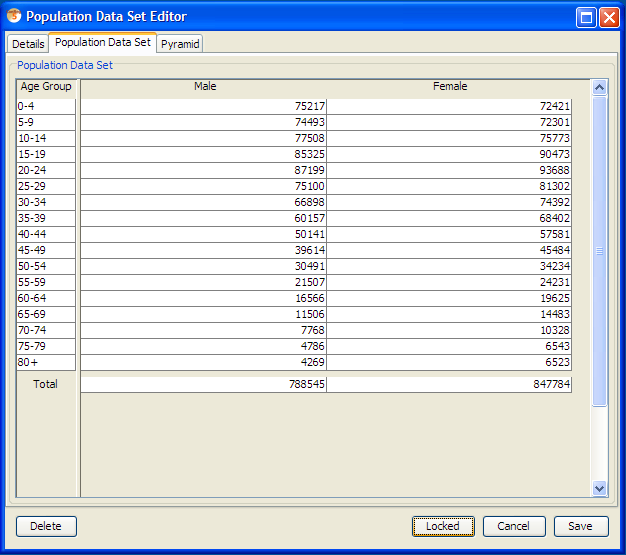
\includegraphics[width=1\columnwidth]{popeditor3}
\par\end{center}

\begin{flushleft}
(Please note that you can copy and paste population datasets back
and forth from general spreadsheets like Excel.) 
\par\end{flushleft}

\begin{flushleft}
Click save to save your population dataset to the database. 
\par\end{flushleft}

You can also take a look at the population pyramid\index{population pyramid}
of the current population data set by going to the Pyramid tab.

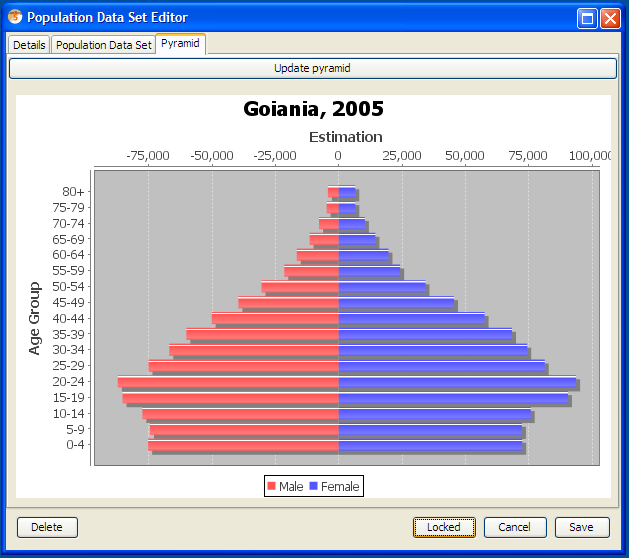
\includegraphics[width=1\columnwidth]{popeditor4-pyram}

This can be saved as an image to disk by right-clicking on the image
and choosing ``Save as PNG...''

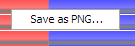
\includegraphics{popeditor4-pyram-save}

And choosing a proper file name.


\subsection{Import population data set\index{import population data set@import\textbf{ }population\textbf{ }data\textbf{ }set}
from CanReg4 }

\begin{flushleft}
Alternatively you can import population data sets from CanReg4\index{CanReg4}.
To do this you go to the Tools menu and choose ``Load CanReg4 Population
Dataset''.
\par\end{flushleft}

\begin{center}
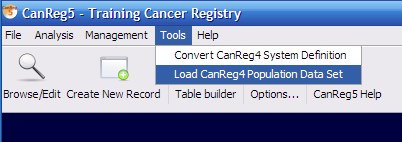
\includegraphics[width=4.1875in,height=1.47917in]{36}
\par\end{center}

\begin{flushleft}
Click Browse to find the population dataset:
\par\end{flushleft}

\begin{center}
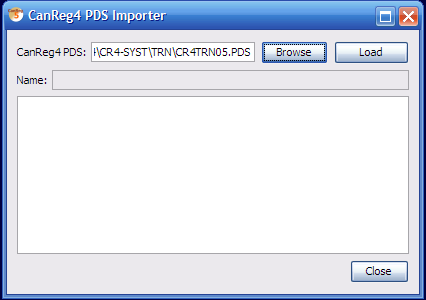
\includegraphics[width=4.4375in,height=3.125in]{37}
\par\end{center}

\begin{flushleft}
Then click Load and a confirmation message that the population dataset
has been loaded will appear.
\par\end{flushleft}

\begin{center}
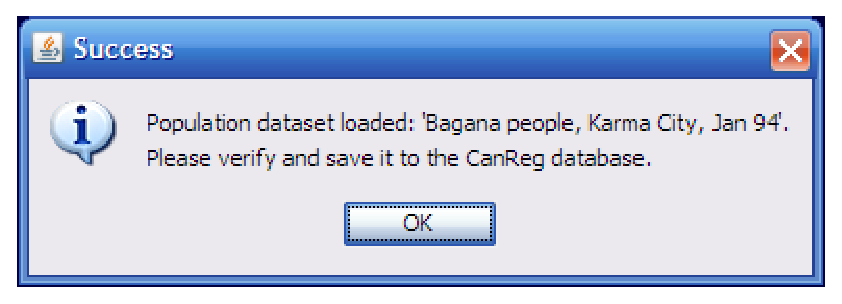
\includegraphics[width=4.04167in,height=1.35417in]{38}
\par\end{center}

\begin{flushleft}
Click ``OK''. 
\par\end{flushleft}

\begin{flushleft}
Next step is to revise the population dataset and see to that it has
been imported correctly.
\par\end{flushleft}

\begin{center}
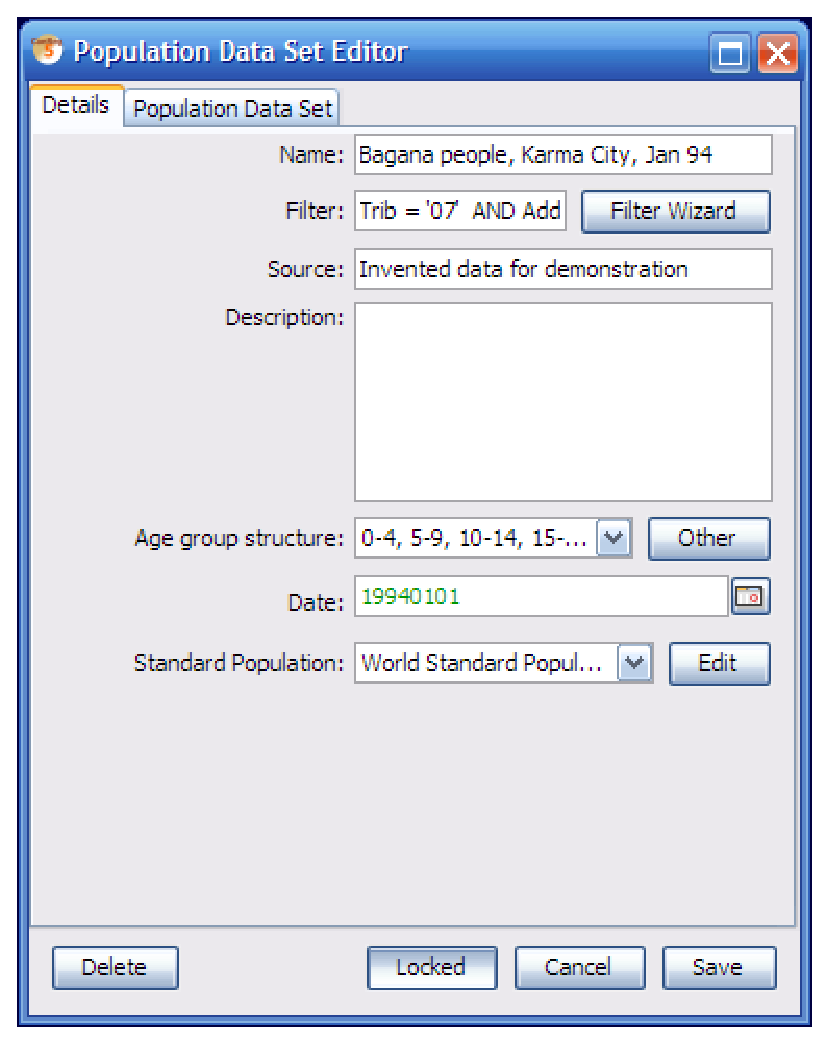
\includegraphics[width=3.97917in,height=5.05208in]{39} 
\par\end{center}

\begin{flushleft}
One important thing to do is to see to that the filter is correct.
That for example the search variables are enclosed by 's. If you need
to change anything in the dataset you need to unlock it by toggling
the ``Locked''-toggle. 
\par\end{flushleft}


\section{Import\index{import}}

The import function lets you import data from other CanReg systems
or other programs.

(For a detailed walk through of how to get the data from CanReg4 to
5 see \vref{sub:Import-the-data}.)

Data in an external file may be added to the CanReg database by importing.
It should be of the following format:
\begin{itemize}
\item Tab delimited\index{tab delimited}
\item Comma Separated Variables\index{comma separated variables}
\item Character delimited\index{character delimited}
\end{itemize}
The easiest way is to have the variable names at the top of each column.

There are four main steps to importing a data file. (If you don't
have all your data in one file, but rather one file per table you
need to repeat the first two steps for each file.)

1) Choose the file(s). 

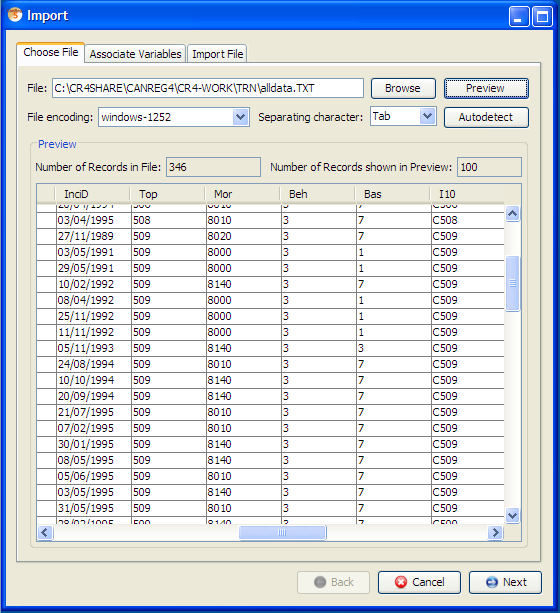
\includegraphics[width=1\columnwidth]{importfilechooser}

Here you also might need to specify the character encoding of your
file as well as the separating chacter used, if CanReg does not detect
it automatically. Please verify using preview.

2) Identify the variables.

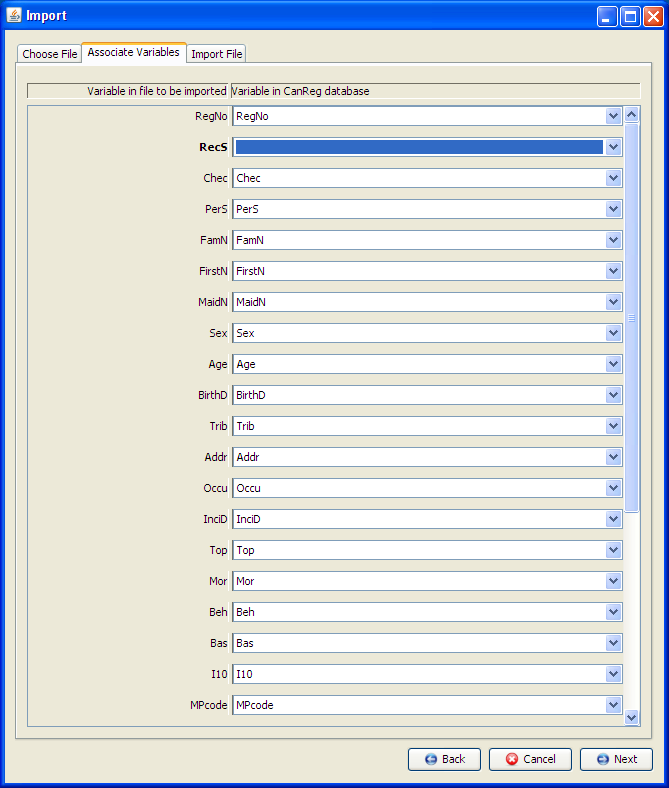
\includegraphics[width=1\columnwidth]{importfileidentifyvariable}

3) Choose the various options - see specific helps.

\includegraphics[width=1\columnwidth]{importfileoptions}

4) Import the file (maybe in \textquotedbl{}test only\textquotedbl{}
mode first)


\subsection{Discrepancies\index{discrepancies}}

A discrepancy is when a record is found with the same registration
number as one in the database, but there are differences in some of
the data.

\includegraphics{importoptionsdiscrepancies}

Click on a \textquotedbl{}radio button\textquotedbl{} to either:
\begin{itemize}
\item Reject these discrepancies (they will not be imported)
\item Update them (any new data will be copied over to the database record)
\item Overwrite (ALL variables will be copied over, even empty ones)
\end{itemize}

\subsection{Max. Lines / Test only}

For testing purposes, you may wish to specify how many lines of the
import file to read.

\includegraphics{importoptionsmaxlines}

With \textquotedbl{}Test only\textquotedbl{} ticked, NO data is actually
added to your database; only a report is generated showing what WOULD
happen. It lists discrepancies, possible matches, rare or error cases
etc.


\subsection{CanReg DATA}

\includegraphics{importoptionscanregdata}


\subsubsection{Perform Checks}

If the data to import was not created using CanReg, or if it is a
Pending case, then the Checks\index{checks} must and will be performed.

If however, the case has already passed the Checks, the Checks will
NOT be performed again unless specified by ticking this option.


\subsubsection{Perform Person Search}

Normally, when importing CanReg data, the Person Search\index{person search}
will still be performed even if already done. If this option is NOT
ticked, then the Person Search will NOT be repeated in this case.
This is only advisable is the case of having no original data.


\subsubsection{Query New First Name}

For data that has not already passed the checks, the First Name\index{name}
and Sex\index{sex} combination will be checked and updated. Tick
this option if you wish all NEW names to be set as pending.

If you are starting a new registry then you probably don't want all
new names to be set as pending, however, if you have several years
of data already, then it would be advisable to query names not already
known.

\newpage{}


\chapter{\index{analysis}Analysis}


\section{Export data\index{export data@export\textsf{\textbf{ }}data}}

To export (write out) all, or part of, your CanReg5 data to an external
text file.

There are two main reasons for doing this:
\begin{itemize}
\item To be able to \emph{import} the file into another program (e.g. \emph{Stata},
\emph{SPSS}, a general spreadsheet like \emph{Excel} or \emph{Calc}
or \emph{Access}) for further analysis.
\item To produce a report, or case listing, that could be read into \emph{Word}
and printed out.
\end{itemize}
\begin{flushleft}
To export your data go to Analysis -> Export Data/Reports:
\par\end{flushleft}

\begin{center}
\includegraphics[width=4.0625in,height=1.52083in]{27}
\par\end{center}

\begin{flushleft}
You will be presented with a screen that resembles the browse-screen:
\par\end{flushleft}

\begin{center}
\includegraphics[width=1\columnwidth]{export}
\par\end{center}

The following steps need to be taken:
\begin{itemize}
\item Specify the records you want to be selected by using the Filter(\vref{sub:Filter})
and Range(\vref{sub:Range}) options, and the order in which they
will be written using the Sort by(\vref{sub:Sorty-by}).
\item Select the Variables(\vref{sub:ExportVariablesSelector}) to display.
\item Choose the Variable headers to include.
\item Choose the File Format (\vref{sub:Export-file-format}) suitable for
your needs.
\end{itemize}
\begin{flushleft}
Please note that some of the functionality, like the ability to store
export-setups is not yet implemented. 
\par\end{flushleft}


\subsection{Options}

\includegraphics{exportoptions}


\subsection{Export file format\index{export file format}\label{sub:Export-file-format}}

All file formats produce text files, with one case per line (a new
line at the end of each case). They all have default extension .TXT
except for \textquotedbl{}Comma Separated Variable\textquotedbl{},
which has .CSV. \textquotedbl{}Tab Delimited\textquotedbl{} writes
each variable separated by the TAB character. \textquotedbl{}Comma
Separated Values\textquotedbl{} encloses each variable in quotes,
and separates by a comma.

\begin{flushleft}
If you export data to a ``Tab Separated'' or a ``Comma Separated''
file you can open this in general spreadsheets (like \emph{Excel}).
\par\end{flushleft}


\subsection{Titles\index{titles}, variable names\index{variable names}}

\includegraphics{exporttitles}


\subsubsection{Titles }

Will write at the top of your export file:
\begin{itemize}
\item the filter criteria, index and ranges used,
\item today's date.
\end{itemize}
This option is useful is you are writing a report, or case listing.
(Not yet implemented.)


\subsubsection{Short variable name }

Puts the abbreviated names of the variables at the top of each column.
(If this file were imported into, for example\emph{ Access} or \emph{R
}then these would automatically become the names of the variables.)


\subsubsection{Long Variable name }

Writes the full name of the variable at the top of each column.


\subsection{Variables\label{sub:ExportVariablesSelector}}

\includegraphics{exportvariables}

Select the variables to export\index{variables to export}.

Tick the boxes next to the variable name to select (or deselect).
They will appear in the data grid after you have clicked refresh table.
(Note that even though you select to export the category names or
descriptions they only show up as codes in the preview window.)

You can drag the grid columns to change the order of the variables.

Click on \textquotedbl{}All variables\textquotedbl{} to select them
all.


\subsection{Date Format}

\includegraphics{exportdateformat}

Tick \textquotedbl{}Format Date\index{format date}\textquotedbl{},
for example, to export \textquotedbl{}21/04/2001\textquotedbl{} instead
of numeric form \textquotedbl{}20010421\textquotedbl{}.

Tick \textquotedbl{}Correct Unknown\index{correct unknown}\textquotedbl{}
so that unknown day will be written as \textquotedbl{}01\textquotedbl{}
and unknown month as \textquotedbl{}07\textquotedbl{}. This is necessary
if you wish to import the data into \emph{Excel}, or any other software
that will reject invalid dates. (Please note that you lose information
on what dates are unknown and what dates are really mid-year.)


\subsection{Export setup}

\includegraphics{exportsetup}

This module is used to load previously made export settings or save
the current settings. This includes the filter, the sequence, the
variables to export and the various options. (Not yet implemented.)


\section{Table builder\index{table builder@table\textsf{\textbf{ }}builder}}

\begin{flushleft}
The Table builder (See figure \vref{fig:Table-builder}) lets you
build incidence tables\index{incidence tables} etc in CanReg. You
find it under analysis --> table builder. 
\par\end{flushleft}

\begin{center}
\begin{figure}
\begin{centering}
\includegraphics[width=4.07292in,height=1.57292in]{40}
\par\end{centering}

\protect\caption{\label{fig:Table-builder-in-the-menu}Table builder in the menu.}
\end{figure}

\par\end{center}


\subsection{Example}

\begin{flushleft}
When you start it you first choose the type of table you want to produce.
(Please note that not all the tables in the list has been implemented.)
\par\end{flushleft}

\begin{flushleft}
Pick Incidence per 100,000 by age group (Period): 
\par\end{flushleft}

\begin{center}
\begin{figure}
\begin{centering}
\includegraphics[width=5.04167in,height=4.125in]{41}
\par\end{centering}

\protect\caption{\label{fig:Table-builder}Table builder}
\end{figure}

\par\end{center}

The incidence rate is defined as:

$\frac{incidence\: cases\: per\: year}{population\: at\: risk}\times10000$

This gives an idea of the risk of getting each type of cancer - the
tables consist of Incidence Rates by Sex, Age group and ICD10\index{ICD10}
cancer type.

\begin{flushleft}
Click on range to set the range of your analysis and set it to match
the analysis you want to do, for example here we want to look at Karma
City, 1991 to 1993: 
\par\end{flushleft}

\begin{center}
\begin{figure}[h]
\begin{centering}
\includegraphics[width=5.02083in,height=4.125in]{42}
\par\end{centering}

\protect\caption{\label{fig:The-range-chooser}The range chooser.}
\end{figure}

\par\end{center}

\begin{flushleft}
In order to create tables of incidence rates, we need to know the
size of the population at risk. Therefore, a \textquotedbl{}Population
Data Set\textquotedbl{} is needed. 
\par\end{flushleft}

\begin{flushleft}
Click ``Population Data Set\index{population data set}\index{PDS}''.
Pick one population data set per year. (Please note that this can
be the same for all three if that year is representative of the period.
See figure \vref{fig:The-population-dataset}.
\par\end{flushleft}

\begin{center}
\begin{figure}[h]
\begin{centering}
\includegraphics[width=5in,height=4.11458in]{43}
\par\end{centering}

\protect\caption{\label{fig:The-population-dataset}The population dataset chooser.}


\end{figure}

\par\end{center}

\begin{flushleft}
Then you can go to the Make tables tab to generate the actual tables.
Click ``Generate post script (PS) files\index{postscript files}''
(See figure \vref{fig:File-formats-selector}.) and choose a file
name. (If the table generates more than one file (like it is the case
for incidence per 100,000 some number or text will be added to the
name you give for each file.) 
\par\end{flushleft}

\begin{center}
\begin{figure}
\begin{centering}
\includegraphics[width=1\columnwidth]{44}
\par\end{centering}

\protect\caption{\label{fig:File-formats-selector}File formats selector}
\end{figure}

\par\end{center}

\begin{flushleft}
You get a message saying, ``Tables built.'' 
\par\end{flushleft}

\begin{flushleft}
Click OK and if you have a program that can read PostScript (See page
\pageref{sub:Tables}.) files the tables will be displayed after you
press OK. (You might have to go to the Orientation menu in \emph{GSView}
and choose Portrait to get the table in the proper orientation.)
\par\end{flushleft}

\begin{center}
\begin{figure}
\begin{centering}
\includegraphics[angle=90,width=0.9\columnwidth]{46}
\par\end{centering}

\protect\caption{\label{fig:Incidence-Rates-per}Incidence Rates per 100.000}
\end{figure}

\par\end{center}


\subsection{File formats}

The various tables can be generated in various file formats, depending
on what they support.


\subsubsection{Portable Document Format (PDF)}

PDF is a well known standard document format that can be read in for
example Adobe Reader, installed on most computers


\subsubsection{Post Script (PS)}

Post Scipt is the predecessor of PDF and is an open format that can
be displayed using for example GSview.


\subsubsection{Scalable Vector Graphics (SVG)}

Scalable Vector Graphics, or SVG, is a scalable editable file format
that lets you further tailor the graphics. This can be viewed in many
programs, incuding most modern internet browsers (as it is part of
the HTML5 standard), and further edited in programs like InkScape
or Adobe Illustrator. They can also be directly embedded in many documents
using Google Docs or Open Office.


\subsubsection{Portable Network Graphics (PNG)}

PNGs are useful for presentation on screen or online, but less adapted
to print, as they are not scalable.


\subsubsection{Windows Meta File (WMF)}

WMFs are useful for presentation on screen, but less adapted to print,
as they are not scalable. (If possible it is better to use PNG as
that is an open format.


\subsubsection{Tabulated data (HTML)}

This is the data from the tables in HTML format for further processing.


\subsection{CanReg5 Chart Editor}

CanReg5 has a built in chart editor for charts that support it. Using
this you can preview and modify the chart before saving it as PNG,
PDF or SVG or printing it. (See figure \vref{fig:CanReg5-chart-editor}.)
\begin{figure}[h]
\begin{centering}
\includegraphics[width=0.6\columnwidth]{charteditor}
\par\end{centering}

\protect\caption{\label{fig:CanReg5-chart-editor}CanReg5 chart editor}
\end{figure}



\subsection{CanReg and SEER{*}Stat\label{sub:CanReg-and-SEER*stat}}

CanReg provides a facility to export data to be used in the free SEER{*}stat\index{SEER{*}Stat}.
(Windows only.) To do so you'll have to first get hold of and install
SEER{*}Stat and SEER{*}Prep\index{SEER{*}Prep} from the SEER website.
(\href{http://seer.cancer.gov/seerprep/}{http://seer.cancer.gov/seerprep/}
and \href{http://seer.cancer.gov/seerstat}{http://seer.cancer.gov/seerstat})

\fbox{\begin{minipage}[t]{1\columnwidth}%
Please note that the following limits apply (for now, as SEER{*}Stat
wants things like this, but in the future we might be able to work
around them):
\begin{itemize}
\item PatientIDs have to be 8 digits or less.
\item Population datasets has to have 5 year age groups.\end{itemize}
%
\end{minipage}}


\subsubsection{In CanReg}

Afterwards you can use the table builder in CanReg and choose the
SEER{*}Prep as table type, specify the range of years you want to
look at, the population datasets matching each year in the period
and click ``Generate files for SEER{*}Prep''. This will ask you
to specify the base name of the files for SEER{*}Prep, i.e. ``Goiania1999-2001''.
(Please note that you can only use ASCII (English) characters in the
paths of the datafiles.) CanReg will add ``cases-'' and ``pop-''
for respectively the incidence file and the population file, as well
as the suffix ``.txd'' so that SEER{*}Prep recognises the files.
CanReg will also create a file describing the data for SEER{*}Prep
- a socalled .dd-file.

Start SEER{*}Prep.


\subsubsection{In SEER{*}Prep}

\begin{figure}
\begin{centering}
\includegraphics[width=0.9\columnwidth]{seerprep}
\par\end{centering}

\protect\caption{SEER{*}Prep in action}
\end{figure}


Load the .dd file you created with CanReg using the little folder
icon.

\fbox{\begin{minipage}[t]{1\columnwidth}%
You can also do this manually. You then have to first specify that
your files follow the NAACCR 1946 v11.3 format, by opening the corresponding
.dd file from the folder you installed SEER{*}prep to. (Most probably
``naaccr1946.ver11\_3.d02032011.dd'') Then under ``Database name:''
you can specify something more instructive than the default.

Then you add your case file and population files from above using
the ``Add...'' buttons.

Do the following choices under ``When Linking to Populations Use:''
\begin{itemize}
\item Age: ``Age recode with <1 years old''
\item Default Std: ``World Std. Million (19 age groups) (recommended)''
\item Race: ``Custom race''
\item Leave Population Count Location as it is (Start col 19, length 8)\end{itemize}
%
\end{minipage}}

Click ``Edit...'' on the study cutoff date for survival and set
it to something after the last entry in the database. (The date of
the export?) (This is not important for now as the survival features
in SEER{*}Stat is not valid for data from CanReg yet.)

Click the ``Lightning'' button. (Or go to the ``Execute'' menu
and choose ``Create file...'' SEER{*}Prep will then ask you where
you want it to write it's report file. Choose somewhere you'll be
able to find it back, i.e. the Desktop. (If you have already created
a database with this name, SEER{*}Prep will ask you if you want to
overwrite it. Choose ``yes'', if you want.)

Next you get some choices regarding invalid values. (The first time
you might want to choose ``Do not exclude any records''.)

That's it. SEER{*}Prep will generate the files that SEER{*}Stat needs.
Exit SEER{*}Prep and start SEER{*}Stat. 

(A more detailed walk through on this process can be found here:

\href{http://seer.cancer.gov/seerprep/example.html}{http://seer.cancer.gov/seerprep/example.html})


\subsubsection{In SEER{*}Stat}

Your data from above should now appear in SEER{*}Stat under the name
you chose for the database above ready to be exploited in SEER{*}Stat. 

You might have to create a new profile, by going to the ``Profile''
menu and choosing ``Add New...''

Click ``Add Local...'' for Data Locations and choose the folder
that SEER{*}Prep writes data to.

(You can also untick the Client-Server ssp-connection if you want.)

Under ``Other variables'' you have to specify valid paths for the
``User Variables'', ``Open or Save'' and ``Temporary Files''.


\section{Frequency distributions\index{frequency distributions}}

\begin{flushleft}
Frequencies distributions let you look at the data in your database
as frequencies by year. You can cross-tabulate\index{cross-tabulate}
several variables. To start this module go to Analysis -- Frequencies
Distributions: 
\par\end{flushleft}

\begin{center}
\includegraphics[width=4.09375in,height=1.41667in]{47}
\par\end{center}

\begin{flushleft}
If you click Refresh table with no filter\index{filter} and no selected
variables you get a table of cases per year.
\par\end{flushleft}

\begin{center}
\includegraphics[width=1\columnwidth]{frequenciesbyyear}
\par\end{center}

\begin{flushleft}
You can sort by any field by clicking its header. For example by number
of cases: 
\par\end{flushleft}

\begin{center}
\includegraphics[width=1.60417in,height=2.94792in]{49}
\par\end{center}

\begin{flushleft}
You can filter the result by adding a filter like for example on incidence
date. You can also add as many variables as you want. 
\par\end{flushleft}

With the save table\index{save table} button you can write the table
to a comma separated file\index{comma separated file} (.CSV\index{CSV})
that can be opened in most porgrams (\emph{Excel}\index{Excel}, \emph{Stata}\index{Stata},
\emph{R}\index{R}...) for further analysis.

\begin{flushleft}
The table can also be selected and copied and pasted into \emph{Excel}\index{Excel},
for example. (No right-click shortcut for that is implemented yet,
but you can select the lines you want and press Ctrl-C (on Windows
and Linux) or Apple-C (on Mac) and paste it into other programs.
\par\end{flushleft}


\subsection{Pivot tables}

\begin{flushleft}
If you save a table with only one stratifier (selected variable) CanReg5
also saves a pivot table based on the data in the table. Here's an
example with the sex variable:
\par\end{flushleft}

\begin{center}
\includegraphics[width=0.75\columnwidth]{pivot-table}
\par\end{center}

\begin{flushleft}
\newpage{}
\par\end{flushleft}


\chapter{Management\index{management}}


\section{Back up and restore}

\begin{flushleft}
Backup\index{backup}-functionality can be found under the Management
menu. 
\par\end{flushleft}


\subsection{Perform backup }

\begin{flushleft}
Under ``Management'' click ``Backup''
\par\end{flushleft}

\begin{center}
\includegraphics[width=4.22917in,height=2.47917in]{22}
\par\end{center}

\begin{flushleft}
Then click ``Perform backup''. This creates the backup of the CanReg5
database on the server machine. If you are on the server machine,
you can see the files you created by clicking ``Open folder containing
Backup\index{folder containing backup}''. It is stored in the \textbf{CanReg
server} folder under Backup and 3 digit code\index{3 digit code}
of the registry and then the date of the backup. On my machine, for
example, it is ``C:\textbackslash{}Documents and Settings\textbackslash{}morten\textbackslash{}.CanRegServer\textbackslash{}Backup\textbackslash{}TRN\textbackslash{}2009-01-14''. 
\par\end{flushleft}


\subsection{Restore from backup\index{restore from backup} }

\begin{flushleft}
If you are on the server machine you can restore the backup you created
above by clicking ``Restore'' in the ``Management''-menu restore
your Registry definition, population dataset, dictionary codes and
any data from a CanReg5 backup.
\par\end{flushleft}

You will probably perform this either:
\begin{itemize}
\item at first installation, or
\item if re-installing on a new computer, or
\item recovering from a lost or damaged computer situation.
\end{itemize}
There are two ways to do this. The easiest one is to use the tool
``Install new system'' that we have access to when CanReg launches.


\subsubsection{Restore with ``Install new system''}

Click ``Install new system'' and browse to the XML file describing
this system and click Open. If this is part of a backup CanReg will
tell you that a backup has been detected and asks you if you want
to restore this. Click yes and it will restore this.


\subsubsection{Restore with ``Restore from backup''-tool}

\begin{center}
\includegraphics[width=4.63542in,height=1.22917in]{23}
\par\end{center}

Simply choose the folder corresponding to the backup you want to restore
using the ``Browse'' button or enter the path manually and the click
``Restore''. You need to specify the folder containing a folder
with a folder named your registry code. That is most of the time the
date of backup. In the example above we restore a backup from january
2009. If you select the folder within this ``date'' folder you will
get an error message and the restore will not be performed.


\section{Manage users\index{manage users@manage\textsf{\textbf{ }}users}}

\begin{flushleft}
The user manager\index{user manager} is located under management
-- users:
\par\end{flushleft}

\begin{center}
\includegraphics[width=4.10417in,height=2.17708in]{29}
\par\end{center}


\subsection{Change your own password }

\begin{flushleft}
To change your own password\index{password}, go to the Current user
tab in the user manager and enter your new password twice. (See figure
\vref{fig:Change-your-own-pqd}.)
\par\end{flushleft}

\begin{center}
\begin{figure}
\begin{centering}
\includegraphics{30}
\par\end{centering}

\protect\caption{\label{fig:Change-your-own-pqd}Change your own password}


\end{figure}

\par\end{center}


\subsection{Database password}

\begin{flushleft}
The CanReg5 database can be encrypted using 56-bit DES encryption.
To enable this you need to provide a minimum 8 characters long password
on the ``Database password'' tab. (See figure \vref{fig:Set-database-password}.)
This protects your database in case somebody gets hold of it. The
user will now be asked for this password everytime she launches the
server. (Once it is running others can connect to the database as
usual.) This is a one way process - the only way to remove the encryption
of your database is to export all the data, build an empty database
and import everything again. The password can, however, be changed
at any point in time.
\par\end{flushleft}

\begin{flushleft}
Please note that if you loose this password you loose access to all
the data in CanReg! (And it is nothing that can be done about it.)
\par\end{flushleft}

\begin{flushleft}
This functionality is only available to users with supervisor access.
\begin{figure}
\begin{centering}
\includegraphics{databasePassword}
\par\end{centering}

\protect\caption{\label{fig:Set-database-password}Set database password}


\end{figure}

\par\end{flushleft}


\subsection{User manager\index{user manager@user\textbf{ }manager} }

\begin{flushleft}
If you are logged in with Supervisor\index{supervisor} rights you
have access to the User manager part of the user manager. (See figure
\vref{fig:User-manager}.) This allows you to add and delete users.
Each user has their own login name\index{login name}, password\index{password}
and permission level\index{permission level}.
\par\end{flushleft}
\begin{itemize}
\item A Supervisor\index{supervisor} can use all options;
\item A Registrar\index{registrar} can perform most of data entry except
to confirm rare cases\index{rare cases} or possible duplicates. Changing
the Dictionary and User Administration (adding users, changing user
levels) are also prohibited.
\item An Analyst\index{analyst} cannot make any changes to the database.
Only analysis options are available.
\end{itemize}
\begin{center}
\begin{figure}
\begin{centering}
\includegraphics{31}
\par\end{centering}

\protect\caption{\label{fig:User-manager}User manager}


\end{figure}

\par\end{center}

\begin{flushleft}
To add a new user, click \textquotedblleft Add user\index{add user}\textquotedblright{}
fill in the user's login name. This will create a default user with
registrar permissions\index{permissions}. To change this select the
user and pick a suitable user right level and click \textquotedblleft Update
user\textquotedblright .
\par\end{flushleft}

\begin{flushleft}
You can change a permission level for a user and hit \textquotedbl{}Update
user\index{update user}\textquotedbl{}, or delete a user\index{delete user}
by selecting the user and then clicking the \textquotedbl{}Delete\textquotedbl{}
button. The default password\index{default password} of any user
is its user name. This should of course be changed at first login
by the user himself.
\par\end{flushleft}


\section{Quality control\index{quality control}}


\subsection{Name and sex}

\includegraphics{nameandsex}

Click the button \textquotedbl{}Show First name\index{name}s by Sex\index{sex}\textquotedbl{}
to view all the names used in your registry:
\begin{itemize}
\item Male names
\item Female names
\item Unisex names (used by both sexes)
\end{itemize}
You should periodically review these lists to check for obvious errors.

New names are automatically added to the lists.

However, if you have made corrections and some names are in the wrong
category, the supervisor can recreate the lists by clicking the second
button. In a network environment, only do this when nobody else is
using the program.


\subsection{Person search\textmd{\index{person search}}}

\includegraphics{duplicatesearch}

Registration number - range start and end.


\subsubsection{Advanced}

Change weights\index{weights} and search variables\index{search variables}.

\includegraphics{advancedduplicatesearch}


\subsubsection{Results}

Results from the search appears here as potential duplicates are found.

\includegraphics{personsearchresults}


\section{Options\index{options}}

\includegraphics{options1}


\subsection{Language\index{language}}

Change language of CanReg5. You need to restart your CanReg5 system
if you change language.


\subsection{Look \& Feel\index{look & feel@look \& feel}}

You need to restart your CanReg5 system if you change font style or
font size.


\subsubsection{Change font}

Set the font size to sizes from Small to Big.


\subsubsection{Change font style}

You can set the font of CanReg by typing the name of the font you
want to use in the Font name text box. (To find out what fonts you
have installed on your Windows system you can take a look at the Fonts
section on your Windows Control Panel.) You can use this if the default
font doesn't contain all the characters you would like to use or if
you just prefer the look of another font.


\subsubsection{Show only outline}

The \textquotedblleft Show only outline\index{only outline} of windows
while moving\textquotedblright{} will increase the performance of
the user interface of CanReg. Tick this if moving windows around the
screen is slow.


\subsection{Periodic backup\index{backup}}

\includegraphics{options12}

Reminder backup options


\subsection{CanReg version\index{CanReg version}}

\includegraphics{options3}

Let the program check to see if the latest version\index{latest version}
of CanReg is installed. This will access the internet to find the
most recent version. You can click ``Download latest version'' to
get the latest universal version of CanReg (The zip-file.) or click
``View Changelog'' to see what is new in CanReg.


\subsection{Paths}

\includegraphics{options4}

Here you can set the paths to the various helper applications of CanReg.
(So far only ``R''.)

\newpage{}

\appendix

\part{Appendix}


\chapter{Frequently asked questions\index{frequently asked questions@frequently\textsf{\textbf{ }}asked\textsf{\textbf{ }}questions}
(FAQ\index{FAQ})}


\section{Server\index{server} }
\begin{description}
\item [{Q:}] \begin{flushleft}
When I click the ``Launch Server\index{launch server}''/``Test
Connection'' button, it takes \textbf{more than 3 minutes} to launch
the server and I get the message that the ``Server {[}is{]} already
running''. Afterwards I cannot log in. 
\par\end{flushleft}
\item [{A:}] \begin{flushleft}
Xenios found the following solution: On our PCs, we use Microsoft
Internet Explorer 7. In the ``Tools / Internet Options / Connections
/ LAN Settings'' we have a tick in the checkbox for ``Use a proxy
server for your LAN'' and the address and port of the proxy server
filled in accordingly. I put a tick in the checkbox for ``Bypass
proxy server for local addresses'', clicked the ``Advanced'' button
and typed the IP address of the PC (localhost) in the ``Do not use
proxy server for addresses beginning with:'' box. 
\par\end{flushleft}
\item [{Q:}] \begin{flushleft}
When I try to log on to the CanReg server I get the message:
``Exception creating connection to: aaa.bbb.ccc.ddd; nested exception
is: java.net.SocketException: Malformed reply from SOCKS server\index{SOCKS server}''
\par\end{flushleft}
\item [{A:}] \begin{flushleft}
This can be solved using the same procedure as the previous
answer.
\par\end{flushleft}
\item [{Q:}] \begin{flushleft}
Is CanReg5 only designed for local networks or does it allow
remote registration\index{remote registration}? 
\par\end{flushleft}
\item [{A:}] \begin{flushleft}
CanReg5 is designed for local networks, yes, but traffic is
over standard TCP/IP\index{TCP/IP} so you can tunnel\index{tunnel}
this through secure channels (SSH\index{SSH}/VPN\index{VPN} etc)
to do remote registration. (This is not \textquotedbl{}officially\textquotedbl{}
supported, as we haven't been able to test it enough (yet).) 
\par\end{flushleft}
\end{description}

\section{Conversion CanReg4\index{CanReg4} to CanReg5\index{conversion CanReg4 to CanReg5}}
\begin{description}
\item [{Q:}] \begin{flushleft}
In what table should the variable age\index{age} be stored?
\par\end{flushleft}
\item [{A:}] \begin{flushleft}
The tumour table. Like that, if the same patient has a new
tumour you can (probably) keep the patient record and just add a new
tumour record. Birth date is stored in the patient table. (Incidence
date with the tumour.) 
\par\end{flushleft}
\item [{Q:}] \begin{flushleft}
Do I need to ``install'' the CanReg5 system definition file
after converting from CanReg4 using the built in tool? 
\par\end{flushleft}
\item [{A:}] \begin{flushleft}
After converting the system you don't need to ``install''
it afterwards as the XML\index{XML} file is automatically copied
to your system folder\index{system folder} during conversion. 
\par\end{flushleft}
\item [{Q:}] \begin{flushleft}
I get errors during import\index{errors during import} of
the data from CanReg4. The process stops after a certain percentage
every time. 
\par\end{flushleft}
\item [{A:}] \begin{flushleft}
Try exporting your data with a comma separated variables\index{comma separated variables}
instead of the default tab-separated ones (or vice versa) and see
if that helps. 
\par\end{flushleft}
\item [{Q:}] \begin{flushleft}
In CanReg5, how do you clear previous data and import fresh
ones from canreg4. 
\par\end{flushleft}
\item [{A:}] \begin{flushleft}
To clear the previous data\index{clear the previous data}
from CanReg5 you need to delete the database files. These can be found
in your user folder\index{user folder} under .CanRegServer\textbackslash{}Database
(On my machine it is under C:\textbackslash{}Documents and Settings\textbackslash{}ervikm\textbackslash{}.CanRegServer\textbackslash{}Database
). Please note that this deletes the dictionaries and population data
as well, so you might want to export those prior to deleting this.
Then you can relaunch CanReg and the server and the empty database
will be rebuilt. It is a good idea to keep a backup of an empty database
- just containing dictionaries (and population data) to get back to
this state of the database if needed.
\par\end{flushleft}
\end{description}

\section{Dictionary\index{dictionary}}
\begin{description}
\item [{Q:}] \begin{flushleft}
Can I import dictionaries\index{import dictionaries} from
other CanReg systems to my own? 
\par\end{flushleft}
\item [{A:}] \begin{flushleft}
Since most CanReg systems have different dictionary structure
(length of codes, order of dictionaries etc.) you need to import the
dictionary corresponding to your system or do necessary modifications. 
\par\end{flushleft}
\end{description}

\section{\label{sub:Tables}Analysis\index{analysis}/tables\index{tables}}
\begin{description}
\item [{Q:}] \begin{flushleft}
What program can I use to view the post script files\index{postscript files}
with? 
\par\end{flushleft}
\item [{A:}] \begin{flushleft}
PostScript is an open standard, so you can use many different
tools to view them. (You can in many cases even send them directly
to a printer.) Apple's OSX and most Linux-distributions (Ubuntu, RedHat,
SuSE etc) come with a tool to view them by default. On Windows the
tool I recommend is the open sourced and free GSview\index{GSview}.
(Available from: \href{http://pages.cs.wisc.edu/~ghost/gsview/}{http://pages.cs.wisc.edu/$\sim$ghost/gsview/}
) To run GS View you need to install Ghostscript\index{Ghostscript}
first. This can be downloaded from here: \href{http://pages.cs.wisc.edu/~ghost/doc/GPL/gpl864.htm}{http://pages.cs.wisc.edu/$\sim$ghost/doc/GPL/gpl864.htm}
(Scroll all the way down, under the heading Microsoft windows and
download the ``GPL Ghostscript 8.64 for 32-bit Windows (the common
variety)'' (\href{http://mirror.cs.wisc.edu/pub/mirrors/ghost/GPL/gs864/gs864w32.exe}{http://mirror.cs.wisc.edu/pub/mirrors/ghost/GPL/gs864/gs864w32.exe})
Run this file to install Ghostscript. Then you can get GSView from
here: \href{http://pages.cs.wisc.edu/~ghost/gsview/get49.htm}{http://pages.cs.wisc.edu/$\sim$ghost/gsview/get49.htm}
(Most probably, you should pick the Win32 self extracting archive
- the first download option. \href{http://mirror.cs.wisc.edu/pub/mirrors/ghost/ghostgum/gsv49w32.exe}{http://mirror.cs.wisc.edu/pub/mirrors/ghost/ghostgum/gsv49w32.exe})
Run this file to install GSView. 
\par\end{flushleft}
\end{description}

\section{Import\index{import}}
\begin{description}
\item [{Q:}] \begin{flushleft}
Some letters are distorted/missing in records after an import.
(For example when importing Arabic names.) Why is that? 
\par\end{flushleft}
\item [{A:}] \begin{flushleft}
If the data is from a program that does not code the data
using Unicode (for example previous versions of CanReg) you need to
specify the coding scheme\index{coding scheme}/``codepage\index{codepage}''
during import of that file to your database. If you pick the wrong
one your data might get distorted. To solve this problem you need
to re-import the data. Please use the preview button during import
to see to that you have the right coding scheme. 
\par\end{flushleft}
\item [{Q:}] \begin{flushleft}
While importing my data the process brakes down before the
end and I get an error message saying that there is something wrong
with the file.
\par\end{flushleft}
\item [{A:}] \begin{flushleft}
First of all make sure that you have the latest version of
CanReg installed, as some of the earlier versions had a bug that manifested
itself while importing files. Then look at the line where the import
brakes down and see if you have some unclosed quotes in any of the
fields. This will brake down the import as CanReg allows qoutes around
strings that contain the separating character, but not unclosed quotes.\\
Another possibility is that your Java Runtime Environment has been
set up with not enough memory. To address this please see \vref{sub:Issues-with-memory}.
\par\end{flushleft}
\end{description}

\section{Database design\index{database design}}
\begin{description}
\item [{Q:}] \begin{flushleft}
What is the minimum data set\index{minimum data set} that
one would collect?
\par\end{flushleft}
\item [{A:}] \begin{flushleft}
The minimum data set required is up to your registry to define.
Please refer to \href{http://www.iarc.fr./en/publications/pdfs-online/epi/sp95/index.php}{this publication}
for more information: (\href{http://www.iarc.fr./en/publications/pdfs-online/epi/sp95/sp95-chap6.pdf}{Chapter 6},
for example. ) The bare minimum are detailed in Figure \vref{fig:Minimum-variables.}.
\begin{figure}
\begin{itemize}
\item Name\index{name}(s): 

\begin{itemize}
\item String, According to local usage, but at least one, eg First name,
Middle name, Last Name, Father's name, Grandfather's name, Maiden
Name.
\end{itemize}
\item Gender/Sex\index{sex}: 

\begin{itemize}
\item Coded, 1 Male; 2 Female; 9 Unknown; (Some registries use 3 for Other.)
\end{itemize}
\item Birth date: 

\begin{itemize}
\item String, Stored in the database as yyyyMMdd (but can, in principle,
be entered in any format), Allows 99 for unknown day and 99 for unknown
month.
\end{itemize}
\item Incidence date: 

\begin{itemize}
\item String, Stored in the database as yyyyMMdd (but can, in principle,
be entered in any format), Allows 99 for unknown day and 99 for unknown
month.
\end{itemize}
\item Address: 

\begin{itemize}
\item Coded, According to local usage/needs.
\end{itemize}
\item Ethnic group (optional, but in some cases encouraged): 

\begin{itemize}
\item Coded, According to local usage/needs.
\end{itemize}
\item Age: 

\begin{itemize}
\item Integer (For legacy reasons this is input as 3 digits, with 999 as
unknown. Some registries collect only two digits so unknown age is
coded as 99 and 98 and greater is coded 98.)
\end{itemize}
\item (Most valid) Basis of diagnosis: 

\begin{itemize}
\item Coded, (1,2,3,4) Non-microscopic, (5,6,7,8) Microscopic, 9 Unknown,
0 Death certificate only.
\end{itemize}
\item Source of information: 

\begin{itemize}
\item Coded, According to local usage, eg hospital number.
\end{itemize}
\item Source of information - additional information: 

\begin{itemize}
\item String, According to local usage, eg hospital record number, name
of physician.
\end{itemize}
\end{itemize}
Note: Registries can choose to collect Date of Birth OR Age, but most
choose to collect both.

\protect\caption{\label{fig:Minimum-variables.}Minimum variables.}
\end{figure}

\par\end{flushleft}
\item [{Q:}] \begin{flushleft}
In what database table\index{database table} should the variable
X be stored?
\par\end{flushleft}
\item [{A:}] \begin{flushleft}
In the \textbf{patient} table\textbf{\index{patient table@patient\textbf{ }table}}
you store the information about the patient that never changes (or
at least very seldom) in the patient table. (That is birth date, sex,
names etc.) You also store follow up information in the patient table.
(Vital status, current address, etc.) In the \textbf{tumour} table\textbf{\index{tumour table@tumour\textbf{ }table}}
you store all data that can potentially differ between two tumours
of the same patient. (Topography, morphology, age, address at the
time of the tumour (coded) etc.) Finally, in the \textbf{source} table
you store all information about the sources of information of any
given tumour. (Source name (preferably coded), source type, date etc.)
\par\end{flushleft}
\item [{Q:}] \begin{flushleft}
After adding a new/removing an old variable to collect in
the database what do I need to do?
\par\end{flushleft}
\item [{A:}] \begin{flushleft}
First of all, before adding or removing variables using the
built in tool or editing the underlying XML file you should take a
backup of your old database. Then you need to export all the data
- one table at a time from CanReg5 - so that you have 3 files. One
for the patient table, one for the tumour table and one for the source
table. Then you need to export the dictionaries. After editing the
database structure you will have to delete the old database files,
relaunch CanReg5 and import these files to the empty database. Basically
what CanReg does when you launch the server is first to load the XML
describing the database, then checks to see if the database files
exist in the Database folder. If this does exist it checks to see
if it corresponds with the XML. If it does not it will not be able
to launch the server. (I'll look into creating a better set of error
messages.) If it does not find a database folder with the registry
code found in the XML it will generate an empty one.
\par\end{flushleft}
\end{description}

\section{Install/update CanReg5\index{database design}}
\begin{description}
\item [{Q:}] \begin{flushleft}
Parts of CanReg5 are no longer working after upgrading to
the latest version. What should I do?
\par\end{flushleft}
\item [{A:}] \begin{flushleft}
First, uninstall CanReg5 and reinstall the latest version.
See if that helps. If not write a bug report to canreg@iarc.fr.\newpage{}
\par\end{flushleft}
\end{description}

\chapter{Known issues}


\section{Known bugs\index{bugs} (errors\index{errors})}
\begin{itemize}
\item \begin{flushleft}
Using a population dataset with a cut off age at less than 85 while
building some R-tables leads to errors in the last age group in the
tables.
\par\end{flushleft}

\begin{itemize}
\item \begin{flushleft}
Severity: Shouldn't cause loss of data 
\par\end{flushleft}
\item \begin{flushleft}
Priority: Medium 
\par\end{flushleft}
\item \begin{flushleft}
Category: Tables
\par\end{flushleft}
\end{itemize}
\end{itemize}

\section{Known limitations\index{limitations}}
\begin{itemize}
\item \begin{flushleft}
You need a population dataset with 5 years age groups for many of
the tables to work properly\ldots{} 
\par\end{flushleft}
\item \begin{flushleft}
Age can not yet be calculated automatically.
\par\end{flushleft}
\item \begin{flushleft}
The result set in the browser is sometimes very slow to scroll around
in. 
\par\end{flushleft}

\begin{itemize}
\item \begin{flushleft}
Solution: Use filters to minimize the number of records shown at any
time or only browse the ``Patient'' or the ``Tumour'' table. 
\par\end{flushleft}
\item \begin{flushleft}
Severity: Shouldn't cause loss of data 
\par\end{flushleft}
\item \begin{flushleft}
Priority: Low 
\par\end{flushleft}
\item \begin{flushleft}
Category: Database/Browse
\par\end{flushleft}
\end{itemize}
\item \begin{flushleft}
\newpage{}
\par\end{flushleft}
\end{itemize}

\chapter{Migrating\index{migrate} from CanReg4\index{CanReg4} - Step by
Step}

(For a video demonstration of this process, please see webinar 3 -
available from the GICR website under ``Resources''. (\href{http://gicr.iarc.fr/en/resources.php\#TRAINING}{http://gicr.iarc.fr/en/resources.php\#{}TRAINING}))

Install CanReg5. (See\vref{sec:Installing-and-running}) Start CanReg5
and it presents you the Welcome window. Do NOT click anything here
just yet.


\section{Step 1 - Import the variable definitions\index{import variable definitions}\index{variable definitions}
of CanReg4 to CanReg5}

The first step is to import the variables of CanReg4 to CanReg5 -
the system definition of CanReg4.)
\begin{enumerate}
\item Go to \textquotedblleft Tool\textquotedblright{} in CanReg5 menu and
click \textquotedblleft Convert system definition\textquotedblright . 

\begin{enumerate}
\item \includegraphics[width=0.9\linewidth]{ToolsConvertCR4Menu}
\end{enumerate}
\item Do \textquotedblleft Browse\textquotedblright{} to find your CanReg4
system definition file. (This is a file located in the folder \textbackslash{}CR4SHARE\textbackslash{}CANREG4\textbackslash{}CR4-SYST\textbackslash{}
followed by your 3 letter registry code i.e. TRN whose name is ending
in .DEF (i.e. CR4-TRN.DEF).) 
\item Select your CanReg4 file and double click it or click \textquotedblleft Open\textquotedblright . 
\item Click \textquotedblleft Convert\textquotedblright . 
\item The program will then ask you if you want to add this server to your
favourites. Click \textquotedblleft Yes\textquotedblright{} here.

\begin{enumerate}
\item \includegraphics[scale=0.5]{5}
\end{enumerate}
\item The next step is the trickiest one during the conversion. Since we
go from a tumour based database structure with only one big table
with all the tumour and patient related information to a structure
with both a table for tumour related information, one for patient
related information and yet another one for source information\eqref{sub:A-short-introduction}
we need to specify what variable goes in what table of CanReg5. We
recommend putting the unique patient related information (name, date
of birth and follow-up variables) in the patient table, source information
in the Source table and pretty much the rest (tumour information,
age, address etc) in the tumour table. 
\item The program presents an initial proposal that you might agree with,
but please go through one by one the variables and decide.

\begin{enumerate}
\item \includegraphics{chooseTableForVariables}
\end{enumerate}
\item Click \textquotedblleft Save\textquotedblright . You have now created
an XML\index{XML} file that describes your CanReg5 system. 
\item Optional: Before you proceed to the next step and launch the server
you can, if you want(!), edit this this XML file you have created.
Either using the built in grapical tool in CanReg5 \eqref{sub:Setting-up-or-modifying}
or manually by opening it in a text editor or a dedicated XML editor.
The file is located in your user folder under .CanRegServer. (On my
machine, for example, running Windows XP it is under: C:\textbackslash{}Documents
and Settings\textbackslash{}morten\textbackslash{}.CanRegServer\textbackslash{}System.)
\item Click \textquotedblleft Login\textquotedblright .
\item Launch the CanReg server 

\begin{enumerate}
\item Click \textquotedblleft Settings\textquotedblright{} 
\item Click \textquotedblleft Launch Server\textquotedblright . (If you
get a java firewall query, please confirm that it is OK that java
can comunicate through you firewall by clicking \textquotedblleft OK\textquotedblright{}
or \textquotedblleft Yes\textquotedblright .) If this is the first
time you launch the server on this machine it will automatically create
the database needed for CanReg5. 
\end{enumerate}
\item Now it is time to log into the system. 

\begin{enumerate}
\item Click \textquotedblleft System\textquotedblright{} 
\item Enter username: \textquotedblleft morten\textquotedblright{} 
\item Enter password: \textquotedblleft ervik\textquotedblright{} 
\item Click \textquotedblleft Login\textquotedblright . The system will
now log you onto your CanReg server. 
\end{enumerate}
\end{enumerate}

\section{Step 2 - Import the dictionary\index{import dictionary}\index{dictionary}
from your CanReg4\index{CanReg4} installation}

The thing we want to do now is to import the \emph{dictionary} from
your CanReg4 installation or demo system. (Earlier we only imported
the description of what variables exist in you canreg4 database.)
This is demonstrated in the video called 06-import-dictionary.avi. 
\begin{enumerate}
\item If you are migrating from CanReg4 make sure to export the most updated
dictionary from your CanReg4 system. (In CanReg4: \textquotedblleft Data
Entry\textquotedblright , \textquotedblleft Dictionary\textquotedblright ,
\textquotedblleft Export dictionary to text file\textquotedblright )
\item Go to \textquotedblleft File\textquotedblright , \textquotedblleft Data
Entry\textquotedblright , \textquotedblleft Edit dictionary\textquotedblright{}
in CanReg5 

\begin{enumerate}
\item \includegraphics[clip]{dictionaryMenu}
\end{enumerate}
\item Click on \textquotedblleft Import complete dictionary from file\textquotedblright . 
\item Browse and select the dictionary from you CanReg4 work folder or elsewhere. 
\item If CanReg does not detect the encoding of the file automatically,
please select it from the drop down list. 
\item Click ``Preview'' to take a look at the dictionary. (Please note
that only the first hundred lines or so are shown.)
\item Tick \textquotedblleft CanReg4 Format\textquotedblright{} if you are
migrating, leave unticked if you are using the demo system or otherwise
are importing a CanReg5 formatted dictionary. 
\item Click ``Import''. This might take some time. Please note the bar
in the lower right indicating that the program is busy. 
\item Afterwards you will receive a message of success imported. Click OK. 
\item Go back to \textquotedblleft File\textquotedblright , \textquotedblleft Data
Entry\textquotedblright , \textquotedblleft Edit dictionary\textquotedblright{}
and verify that the dictionaries have been imported. 
\end{enumerate}

\section{Step 3 - Import the data\index{import data from CanReg4}\index{import data}
from your CanReg4\index{CanReg4} installation}

The next step is to import the \emph{data} from CanReg4 to CanReg5.
This is demoed in the video called 07-import-data.avi.
\begin{enumerate}
\item Make sure you export the most updated data from your CanReg4 system. 

\begin{enumerate}
\item In CanReg4: \textquotedblleft Analysis\textquotedblright , \textquotedblleft Export
data\textquotedblright{} 
\item Tick \textquotedblleft Export all variables\textquotedblright . 
\item Choose variables names short 
\item Under \textquotedblleft Export File options\textquotedblright{} choose
\textquotedblleft Comma separated variables\textquotedblright{} 
\item Untick \textquotedblleft Format date\textquotedblright{} 
\item Untick \textquotedblleft Correct Unknown\textquotedblright{} 
\item Click \textquotedblleft write data to file\textquotedblright{} and
pick a file name that you can find back easily in CanReg5. For example
on the desktop. Click \textquotedblleft save\textquotedblright . 
\item Take a look at the data you have now exported and close CanReg4.
\item Take a note of the number of records. (This should later match the
number of \emph{Tumour records} in your CanReg5 system.)
\end{enumerate}
\item Back in CanReg5 do \textquotedblleft File\textquotedblright , \textquotedblleft Data
Entry\textquotedblright{} and \textquotedblleft Import Data\textquotedblright .
\item Click \textquotedblleft Browse\textquotedblright{} and locate the
file from step A. Select it and click \textquotedblleft Open\textquotedblright .
You can if you want preview the file to see that you picked the right
one and that the file looks OK. If for example Arabic names are garbled
you should try to choose another \textquotedblleft File encoding\textquotedblright{}
(Default for Arabic text is ISO-8859-6).
\item Set \textquotedblleft Separating character\textquotedblright{} to
Comma. (Or whatever separating character your file has.) 
\item Click Preview to see that the data looks OK. 
\item Click \textquotedblleft Next\textquotedblright{} (or select the tab
\textquotedblleft Associate Variables\textquotedblright ) 
\item This lets you associate the variables in the file to import with the
variables in the database. CanReg5 will find most of these associations
by itself, but you should revise them to see if they look OK. Look
for variable names in bold, as they are the one that are not assigned
at all. 
\item Click \textquotedblleft Next\textquotedblright{} (or select the tab
\textquotedblleft Import File\textquotedblright ) 
\item Click \textquotedblleft Import\textquotedblright{} (leave everything
as by default \textendash{} the import function only works on empty
CanReg databases as per now\dots ) 
\item Let CanReg5 import the data (this might take a while) and click \textquotedblleft OK\textquotedblright . 
\item Click \textquotedblleft Browse/Edit\textquotedblright{} and \textquotedblleft Refresh
Table\textquotedblright{} to see that the data has arrived well. \emph{Verify
that you have the same number of tumours in the tumour table as in
CanReg4.} Double click a record to take a look at it.\newpage{}
\end{enumerate}

\chapter{Advanced database management}

This appendix covers some advanced database management topics


\section{The System definition file (the XML file)}


\subsection{Advanced options in the CanReg5 person search}

You have access to a couple of extra settings in the CanReg5 system
definition file to improve the detection of duplicate patients (in
addition to \emph{weight}), namely \emph{discriminatory power, reliability},
and \emph{presence}.


\subsubsection{Weight}

The weight of the link. These can add up to more/less than 100 (but
will then be normalized to 100). The weight is the score that the
link will get if there is a 100\% match on that variable. Some algorithms
also return numbers between 0 and a 100, and if so, the score is adjusted.


\subsubsection{Disciminatory power}

Does nothing at the moment!

(Discriminatory Power calculator: \href{http://insilico.ehu.es/mini_tools/discriminatory_power/index.php}{http://insilico.ehu.es/mini\_{}tools/discriminatory\_{}power/index.php})


\subsubsection{Reliablity}

Does nothing at the moment!

How reliable is the data. Scale from 0 to 1.


\subsubsection{Prescence}

Does nothing at the moment!

How often is the variable filled. Scale from 0 to 1.


\subsubsection{Threshold}

Set between 0 and 100. Cases with higher match percentage than this
shows up in person search.


\chapter{Technical details on the Table Builder}

The graphical tool to build tables in CanReg5, the Table Builder,
can be modified to suit particular needs of users via configuration
files. CanReg comes with some default ones, but these can be added
to as the user sees fit.


\section{Configuration files}

The default configuration files of these tables can be found in the
``conf/tables'' folder in your CanReg5 installation. The user provided
ones are found in the ``conf/tables'' folder in the ``.CanRegClient''
folder. For each line in the Table Builder you will find a corresponding
.conf-file. (See figure \ref{fig:The-Table-Builder})
\begin{figure}
\begin{centering}
\includegraphics{41}
\par\end{centering}

\protect\caption{\label{fig:The-Table-Builder}The Table Builder}


\end{figure}


The user can change or add new configuration files and they will appear
in this list. 


\subsection{The file structure and parameters}

The easiest way to familiarize oneself with the structure of these
configuration files is to open one and take a look. The first thing
we notice is that you have several parameters and labels grouped by
curly brackets. The entry \emph{``table\_label''} for example contains
one entry witch is the label, or name, of the table. This is what
will be displayed in the list in the table builder. Let's go through
the standard groups one by one:


\subsubsection{table\_label}

The name or label of the table.


\subsubsection{table\_description}

The description of the table - more information that the user will
see when he selects the table in the list.


\subsubsection{table\_engine}

This is the name of the engine that will produce the table when the
user click \emph{Generate }in CanReg5\emph{.} More on this in the
next sub section.


\subsubsection{engine\_parameters}

These are parameters to the different engines, and can be anything
the engine understand. For example a code saying ``noC44'' to tell
the engine that this should be counts exluding skin cancer - if the
engine supports that parameter.


\subsubsection{preview\_image}

This is the name of a file found in one of the previews folders (within
the ``conf/tables'' folders mentioned above) that will displayed
in CanReg when the user has selected this table. The user provided
previews override the system provided ones.


\subsubsection{ICD\_groups\_labels}

Many tables also need a list of ICD group labels to display. This
is just a list of labels with the 3 first characters detailing if
this should be displayed for male/female cases. For example the line:
\begin{lyxcode}
\textquotedbl{}11~Lip\textquotedbl{}
\end{lyxcode}
Means that the name of this site/group of sites is Lip and it should
be displayed for both male and female.
\begin{lyxcode}
\textquotedbl{}01~Ovary\textquotedbl{}
\end{lyxcode}
on the other hand means that this should only be displayed for female
cases.


\subsubsection{ICD10\_groups (or ICD\_groups)}

Each of the labels from ICD\_groups\_labels must have a corresponding
definition detailing the actual ICD10 codes that goes into this group.
This can be found in ICD10\_groups. Line number 1 in ICD\_groups\_labels
corresponds to line 1 in ICD10\_groups, line 2 to line 2 etc. These
groups are parsed and interpreted run-time by CanReg so you can define
your own groups by following the following rules:
\begin{enumerate}
\item For a single site enter the ICD10 code for that site, i.e. ``C09''.
\item For a single subsite enter the ICD10 code for that site, i.e. ``C000''.
\item For a range enter it as <site>-<site without the leading 'C'>, i.e.
\textquotedbl{}C30-31\textquotedbl{}.
\item For a series of sites enter them like <site or range>, <site or range>
etc., i.e. \textquotedbl{}C47,C49\textquotedbl{} or \textquotedbl{}C82-85,C96\textquotedbl{}
\item There are some special sites that can be defined by using their standard
names. These can not be part of any range or series:

\begin{enumerate}
\item \textquotedbl{}MPD\textquotedbl{} - Myeloproliferative disorders
\item \textquotedbl{}MDS\textquotedbl{} - Myelodysplastic syndromes
\item \textquotedbl{}O\&U\textquotedbl{} - Other and unspecified
\item \textquotedbl{}ALL\textquotedbl{} - All sites
\item \textquotedbl{}ALLbC44\textquotedbl{} - All sites but C44
\end{enumerate}
\end{enumerate}

\section{Engines}

CanReg5 has an ever increasing number of built in engines to produce
tables. Their names:
\begin{itemize}
\item ``incidencerates''
\item ``numberofcases''
\item ``populationpyramids''
\item ``top10piechart''
\item ``r-engine''
\item \textquotedbl{}r-engine-grouped\textquotedbl{}
\end{itemize}

\subsection{Incidence Rates Table(``incidencerates'')}

This is the engine that produces a A4 ready to print overview of number
of cases per 100.000 per site in the database. (See figure \vref{fig:Incidence-Rates-per}.)


\subsubsection{line\_breaks}

One special parameter in the configuration file of this table is the
line\_breaks. It is a list of pairs of numbers detailing where to
put grey boxes behind the numbers to make them easier to read. For
example
\begin{lyxcode}
\textquotedbl{}8,9\textquotedbl{}

\textquotedbl{}17,-1\textquotedbl{}

\textquotedbl{}21,1\textquotedbl{}
\end{lyxcode}
This means that at line 8 we start a 9 line big box. Stopping at line
17. Picks up again on line 21 for just one line.


\subsection{Number of Cases (``number of cases'')}

This is the engine that produces a A4 ready to print overview of number
of cases per site in the database.


\subsubsection{line\_breaks}

This has the same special parameter line\_breaks as the ``incidencerates''
engine.


\subsection{Population Pyramids (``populationpyramids'')}

This is the simplest configuration file so far as it looks like this:
\begin{lyxcode}
table\_label~\{
\begin{lyxcode}
\textquotedbl{}Population~Pyramids\textquotedbl{}~

\}
\end{lyxcode}
table\_description~\{
\begin{lyxcode}
\textquotedbl{}Population~Pyramids\textquotedbl{}~

\}
\end{lyxcode}
table\_engine~\{
\begin{lyxcode}
\textquotedbl{}populationpyramids\textquotedbl{}~

\}
\end{lyxcode}
preview\_image~\{
\begin{lyxcode}
\textquotedbl{}populationpyramid.png\textquotedbl{}~

\}~
\end{lyxcode}
\end{lyxcode}

\subsection{Top 10 pie chart (``top10piechart'')}

\begin{figure}[h]
\includegraphics[width=1\linewidth]{pieChart}

\protect\caption{\label{fig:Pie-Chart}Pie Chart}


\end{figure}


Here you place your ``candidate'' groups in the ICD10\_groups and
ICD\_groups\_labels in the .conf file and the engine produses a pie
chart of the 10 most common cancers in your registry for the period
you have provided in either PNGs or SVGs. (See\vref{fig:Pie-Chart})

If you pass ``noC44'' as one of the engine parameters you get tables
excluding skin cancer.


\subsection{The R engines (``r-engine'' and ``r-engine-grouped'')}

You can call R programs directly from within the TableBuilder of CanReg5.
This is detailed in \vref{sub:CanReg-and-R}.


\section{\label{sub:CanReg-and-R}CanReg and R\index{R}}


\subsection{Configuration file parameters}

Like with the other Table Builder engines of CanReg you can configure
the R engines as well using configuration files. Specific to the R
engines are the following parameters:


\subsubsection{r\_scripts}

This can be one or many R scripts that gets called by CanReg to produce
tables. (See the listing on page \pageref{A-sample-main} for a skeleton
script.)


\subsubsection{file\_types\_generated}

This details what filetypes this R script can generate. For example:
\begin{lyxcode}
file\_types\_generated~\{~
\begin{lyxcode}
\textquotedbl{}pdf\textquotedbl{}~

\textquotedbl{}ps\textquotedbl{}~

\textquotedbl{}svg\textquotedbl{}

\textquotedbl{}html\textquotedbl{}

\}
\end{lyxcode}
\end{lyxcode}
\label{A-sample-main}\lstset{language=R}
\lstset{backgroundcolor=\color{lightyellow}}
\lstset{caption=A sample main R script (See the folder conf/tables/r for more info)}
\begin{lstlisting}[frame=tb]
Args <- commandArgs(TRUE)
## Find directory of script 
initial.options <- commandArgs(trailingOnly = FALSE) 
file.arg.name <- "--file=" 
script.name <- sub(file.arg.name, "", 
initial.options[grep(file.arg.name, initial.options)]) 
script.basename <- dirname(script.name) 

source(paste(sep="/", script.basename, "makeTable.R")) 
source(paste(sep="/", script.basename, "checkArgs.R")) 
source(paste(sep="/", script.basename, "makeFile.R"))

##OutFile out <- checkArgs(Args, "-out")
fileType <- checkArgs(Args, "-ft")

# Load dependencies 
source(paste(sep="/", script.basename, "myLibrary1.R"))
...
source(paste(sep="/", script.basename, "myLibraryN.r"))

# The incidence file  
fileInc <- checkArgs(Args, "-inc") 
dataInc <- read.table(fileInc, header=TRUE)

# The population file 
filePop <- checkArgs(Args, "-pop")
dataPop <- read.table(filePop, header=TRUE)

#do your plot
generatedFilenames = createMyNiceFigure(dataInc, dataPop) 
dev.off()

# write the name of any file created by R to out 
cat(generatedFilenames)
\end{lstlisting}
\lstset{backgroundcolor=\color{white}}
\lstset{language= , caption= }


\subsection{Arguments}

When calling the R scripts CanReg provides the following arguments:
\begin{itemize}
\item \emph{-ft=<filetype>} The file type - either pdf, png, wmf, ps, html
or svg.

\begin{itemize}
\item This is how CanReg gives information to the R program on what file(s)
should be created.
\end{itemize}
\item \emph{-out=<filename>} The base of the report file name - or output
file name if you want.

\begin{itemize}
\item The R program generates either a file with that name - with added
standard file type suffix, or a series of file names with this as
the base. One important point is that the way CanReg detects what
files that actually has been created is by listening to the standard
output of R. All the R program has to do is to write (print or cat)
the files generated to standard out and CanReg will try to do system
calls to display them when they are done.
\end{itemize}
\item \emph{-pop=<filename>} Population file name. 
\item \emph{-inc=<filename>} Incidence file name.
\end{itemize}
Some scripts can also take additional arguments like:
\begin{itemize}
\item \emph{-logr }Turn\emph{ }logaritmic plots on.
\item \emph{-onePage=axb} Generate summary page(s) with all the plots laid
out in a columns and b rows.
\end{itemize}
Example call: 
\begin{lyxcode}
\textquotedbl{}C:\textbackslash{}Program~Files\textbackslash{}R\textbackslash{}R-2.12.2\textbackslash{}bin\textbackslash{}R.exe\textquotedbl{}~

-{}-slave~-{}-file=

\textquotedbl{}C:\textbackslash{}Users\textbackslash{}ervikm\textbackslash{}Desktop\textbackslash{}CanReg\textbackslash{}.\textbackslash{}conf\textbackslash{}tables\textbackslash{}r\textbackslash{}test.r\textquotedbl{}

-{}-args~-ft=svg~-out=\textquotedbl{}C:\textbackslash{}Documents~and~Settings\textbackslash{}ervikm\textbackslash{}Desktop\textbackslash{}test\textquotedbl{}

-pop=\textquotedbl{}C:\textbackslash{}Users\textbackslash{}ervikm\textbackslash{}Temp\textbackslash{}pop4834689295162083243.tsv\textquotedbl{}

-inc=\textquotedbl{}C:\textbackslash{}Users\textbackslash{}ervikm\textbackslash{}Temp\textbackslash{}inc4297000362541616146.tsv\textquotedbl{}

-onePage=3x4~
\end{lyxcode}
(The user never sees this, but it can be useful to keep this in mind
when writing your own R scripts.)


\subsection{Population file }

CanReg writes a population file to a temporary file with the following
columns:
\begin{enumerate}
\item YEAR 
\item AGE\_GROUP\_LABEL 
\item AGE\_GROUP 
\item SEX 
\item COUNT
\end{enumerate}

\subsection{Incidence file}

CanReg writes an incidence file to a temporary file with a structure
depending on the script and the engine.


\subsubsection{r-engine}

If you use the r-engine you can specify the columns you need from
CanReg with the variables\_needed configuration file parameter. For
example:
\begin{lyxcode}
variables\_needed~\{~
\begin{lyxcode}
\textquotedbl{}Age\textquotedbl{}~

\textquotedbl{}ICD10\textquotedbl{}~

\textquotedbl{}Sex\textquotedbl{}~

\}
\end{lyxcode}
\end{lyxcode}
This will create an incidence file with the following columns: 
\begin{enumerate}
\item YEAR (added automatically)
\item AGE
\item ICD10
\item SEX
\item CASES (added automatically)
\end{enumerate}

\subsubsection{r-engine-grouped}

If you use the grouped version of the r-engine CanReg will group the
cancer cases according to the groups defined in the configuration
file and create an incidence file with the following columns:
\begin{enumerate}
\item YEAR 
\item ICD10GROUP
\item ICD10GROUPLABEL
\item SEX 
\item AGEGROUP 
\item MORPHOLOGY
\item BEHAVIOUR 
\item BASIS 
\item CASES
\end{enumerate}

\subsection{SVG support}

To be able to generate SVG files in the R programs you need to install
a package called ``RSvgDevice'' from within R. To install this package
you need to lauch R and type in the following command.
\begin{lyxcode}
install.packages(\textquotedbl{}RSvgDevice\textquotedbl{})
\end{lyxcode}
Then select a country (mirror) close to you and click OK. This will
install the package and it is ready for R to use. You can now close
R and if all went well start producing SVG figures calling R functions
from CanReg.

(In the latest version of the R programs distributed with CanReg there's
built in functionality to automatically install this package if you
are connected to the internet.)

\newpage{}


\chapter{Third party tools}

Here's a list of useful free third-party tools to use with CanReg5.


\section{Java Runtime Environment}

To run CanReg at all you need a Java Runtime Environment\index{Java Runtime Environment}.
You can get it from \href{http://java.com/en/download/manual.jsp}{http://java.com/en/download/manual.jsp}.


\subsection{\label{sub:Issues-with-memory}Issues with memory}

By default most JVM implementations limit themselves to using a small
amount of RAM (eg: 64MB), even if your computer has a lot of system
RAM (eg: 1GB). This can lead to out of memory conditions, even if
your computer has lots of free memory. To configure your JVM to use
more memory, complete the following steps:


\subsubsection{On Windows:}

Go to Control Panel | Java , in 'Java' panel, click view Java applet
running settings. Set Java Running Parameters to:

-Xmx256M -Xms256M -Xss128k

Save and apply these changes. You must close and restart CanReg (and
potential web browsers open) for these changes to take effect.

These settings require 256MB of contiguous memory be available. You
may need to restart your computer before these settings will work.


\subsubsection{On Solaris/Linux:}
\begin{lyxcode}
cd~/bin~

./ControlPanel~
\end{lyxcode}
Change Java Applet running Parameters to: -Xmx256M -Xms256M -Xss128k

Press OK, restart CanReg (and potential web browsers open) for these
changes to take effect.

This will configure your JVM to use a fixed 256MB of RAM.

If you have multiple versions of java on same machine, please perform
the above operations for all versions. 


\section{Analysis}


\subsection{\label{sub:R}R}

R is a free software environment for statistical computing and graphics.
It compiles and runs on a wide variety of UNIX platforms, Windows
and MacOS.

More information about it on: \href{http://www.r-project.org/}{http://www.r-project.org/}

To download R\index{R} go to \href{http://cran.r-project.org/mirrors.html}{http://cran.r-project.org/mirrors.html}
and choose a mirror near you, for example \href{http://cran.univ-lyon1.fr/}{http://cran.univ-lyon1.fr/}.
Choose your platform, i.e. Windows, click the link that says ``base'',
i.e. \href{http://cran.univ-lyon1.fr/bin/windows/base/}{http://cran.univ-lyon1.fr/bin/windows/base/}
and then click ``Download R...''. The latest as of the 25th of September
2013 is version 3.0.2 and you can get more information on the installation
procedure here: \url{http://cran.r-project.org/src/base/NEWS.html}.


\subsection{Epi Info}

From the Epi Info\index{Epi Info} website: 
\begin{quote}
``Physicians, nurses, epidemiologists, and other public health workers
lacking a background in information technology often have a need for
simple tools that allow the rapid creation of data collection instruments
and data analysis, visualization, and reporting using epidemiologic
methods. Epi Info\texttrademark , a suite of lightweight software
tools, delivers core ad-hoc epidemiologic functionality without the
complexity or expense of large, enterprise applications.''
\end{quote}
More information about it on: \href{http://wwwn.cdc.gov/epiinfo/}{http://wwwn.cdc.gov/epiinfo/}

The newest version of EpiInfo is windows based, but CDC also provides
a DOS based version, Epi Info 6. (Available here: \url{http://wwwn.cdc.gov/epiinfo/html/ei6_downloads.htm}.
)


\subsection{SEER{*}Stat and SEER{*}Prep}

From the SEER website:
\begin{quote}
``The SEER{*}Stat\index{SEER{*}Stat} statistical software provides
a convenient, intuitive mechanism for the analysis of SEER and other
cancer-related databases. It is a powerful PC tool to view individual
cancer records and to produce statistics for studying the impact of
cancer on a population.''
\end{quote}
To get your data from CanReg to SEER{*}Stat you need to go via SEER{*}Prep\index{SEER{*}Prep}.
(See \vref{sub:CanReg-and-SEER*stat} for more information.)


\subsection{PSPP}

``PSPP is a program for statistical analysis of sampled data. It
is a Free replacement for the proprietary program SPSS, and appears
very similar to it with a few exceptions.'' Available from \href{http://www.gnu.org/software/pspp/}{http://www.gnu.org/software/pspp/}.


\subsection{SOFA}

SOFA - Statistics Open For All The user-friendly, open-source statistics,
analysis, and reporting package. Available from \href{http://www.sofastatistics.com/home.php}{http://www.sofastatistics.com/home.php}.


\section{Data cleaning and record linkage\index{data cleaning}}


\subsection{Google Refine\index{Google Refine}}

Google Refine is a free and open source tool that allows you to standardise
and clean your data prior to importing it into CanReg5. Please note
that even though you access and manipulate your data using a web browser
your data is kept locally on your machine. 

More information about it on: \href{http://code.google.com/p/google-refine/}{http://code.google.com/p/google-refine/}


\subsection{Talend Open Studio\index{Talend Open Studio}}

Talend Open Studio is a more heavy duty package to clean and standardise
your data before importing it into CanReg. It is free and open source. 

More information about it on: \href{http://www.talend.com/}{http://www.talend.com/}


\subsection{FRIL: Fine-Grained Records Integration and Linkage Tool}

From their website:
\begin{quote}
``FRIL is FREE open source tool that enables fast and easy record
linkage. The tool extends traditional record linkage tools with a
richer set of parameters. Users may systematically and iteratively
explore the optimal combination of parameter values to enhance linking
performance and accuracy. ``
\end{quote}
More information about it on: \href{http://fril.sourceforge.net/index.html}{http://fril.sourceforge.net/index.html}


\subsection{LinkPlus}

From the CDC website:
\begin{quote}
``Link Plus is a probabilistic record linkage program developed at
CDC's Division of Cancer Prevention and Control in support of CDC's
National Program of Cancer Registries (NPCR). Link Plus is a record
linkage tool for cancer registries. It is an easy-to-use, standalone
application for Microsoft\textregistered{} Windows\textregistered{}
that can run in two modes\textemdash{}

To detect duplicates in a cancer registry database. To link a cancer
registry file with external files. Although originally designed to
be used by cancer registries, the program can be used with any type
of data in fixed width or delimited format. Used extensively across
a diversity of research disciplines, Link Plus is rapidly becoming
an essential linkage tool for researchers and organizations that maintain
public health data.''
\end{quote}
More information about it on:\url{http://www.cdc.gov/cancer/npcr/tools/registryplus/lp.htm}


\section{Data security\index{data security}}


\subsection{GnuPG\index{GnuPG}}
\begin{itemize}
\item Complete and free implementation of the OpenPGP standard. (\href{http://gnupg.org/}{http://gnupg.org/})
\item Allows to encrypt and sign your data and communication. 
\item Easy to use and set up. 
\item OS independant 

\begin{itemize}
\item Gpg4win on Windows \href{http://www.gpg4win.org}{http://www.gpg4win.org}
\item GPGTools on Mac OS X 
\end{itemize}
\item Integrates with email clients 

\begin{itemize}
\item Enigmail
\end{itemize}
\end{itemize}

\subsection{TrueCrypt\index{TrueCrypt}}
\begin{itemize}
\item Free open-source disk encryption\index{disk encryption} software. 
\item On-the-fly-encrypted volume (data storage device). 
\item For Windows 7/Vista/XP, Mac OS X, and Linux.
\item \href{http://www.truecrypt.org}{http://www.truecrypt.org}
\end{itemize}

\section{Graphics display/editing}


\subsection{\label{sub:PostScript-Viewer}PostScript Viewer\index{postscript viewer@postscript\textbf{ }viewer}
\index{PS files}}

\begin{flushleft}
Some of the tables generated by CanReg5 are PostScipt files\index{postscipt files}.
PostScript is an open standard, so you can use many different tools
to view them. (You can in many cases even send them directly to a
printer.) Mac OS X and most Linux-distributions come with tools to
view them by default. 
\par\end{flushleft}

\begin{flushleft}
On Windows, the tool I recommend is the open sourced and free GSview\index{GSview}. 
\par\end{flushleft}

\begin{flushleft}
To run GS View you need to install \index{Ghostscript}Ghostscript
first. This can be for example be downloaded from here: \href{http://pages.cs.wisc.edu/~ghost/doc/GPL/gpl900.htm}{http://pages.cs.wisc.edu/$\sim$ghost/doc/GPL/gpl900.htm}
(Scroll all the way down, under the heading Microsoft windows and
download the ``GPL Ghostscript 9.00 for 32-bit Windows (the common
variety)'' (\href{http://mirror.cs.wisc.edu/pub/mirrors/ghost/GPL/gs900/gs900w32.exe}{http://mirror.cs.wisc.edu/pub/mirrors/ghost/GPL/gs900/gs900w32.exe}) 
\par\end{flushleft}

\begin{flushleft}
Run this file to install Ghostscript.
\par\end{flushleft}

\begin{flushleft}
Then you can get GS View from here: \href{http://pages.cs.wisc.edu/~ghost/gsview/get49.htm}{http://pages.cs.wisc.edu/$\sim$ghost/gsview/get49.htm}
(Most probably, you should pick the Win32 self extracting archive
- the first download option. \href{http://mirror.cs.wisc.edu/pub/mirrors/ghost/ghostgum/gsv49w32.exe}{http://mirror.cs.wisc.edu/pub/mirrors/ghost/ghostgum/gsv49w32.exe}) 
\par\end{flushleft}

\begin{flushleft}
Run this file to install GS View. 
\par\end{flushleft}


\subsection{InkScape}

InkScape is a free open source program to display and edit SVGs and
other vector based files. 

From their website: 
\begin{quote}
``An Open Source vector graphics editor, with capabilities similar
to Illustrator, CorelDraw, or Xara X, using the W3C standard Scalable
Vector Graphics (SVG) file format.

Inkscape supports many advanced SVG features (markers, clones, alpha
blending, etc.) and great care is taken in designing a streamlined
interface. It is very easy to edit nodes, perform complex path operations,
trace bitmaps and much more.''
\end{quote}
Available from: \href{http://inkscape.org/}{http://inkscape.org/}


\section{General}


\subsection{Notepad++}

Notepad++ is an excellent open source text editor that is perfect
for writing code, cleaning a dataset using, for example regular expressions,
or just simply looking at data from CanReg. Available from: \href{http://notepad-plus-plus.org/}{http://notepad-plus-plus.org/}
(It has nothing to do with the Notepad that is distributed with Windows
- it merely shares the first part of it's name with it.)

\newpage{}


\chapter{Scripts}


\section{Ruby scripts}


\subsection{Script to generate icd10 codes and cancer groups}

This tool lets you add icd10 codes and user defined groups to data
in a csv file.


\subsubsection{Prerequisites}


\paragraph{Install JRuby }
\begin{enumerate}
\item Downoad the latest JRuby from here: http://jruby.org/download fitting
your machine 
\item Run the installer and follow on screen instructions. (Make sure you
add jruby to the path when asked.)
\item Windows: Run the ``install.bat'' in the script folder. Linux/Mac:
run the following commands:\end{enumerate}
\begin{lyxcode}
jgem~install~bundler~

jruby~-{}-1.9~-S~bundle~install
\end{lyxcode}

\subsubsection{Usage}
\begin{lyxcode}
jruby~-{}-1.9~icd10grouper.rb~{[}options{]}~
\end{lyxcode}

\paragraph{Example: }
\begin{lyxcode}
jruby~-{}-1.9~icd10grouper.rb~-t~Topography~-m~Morphology~-b~Behaviour~

-s~Sex~-c~,~-g~Groups.conf~-f~LotsOfData.csv
\end{lyxcode}

\paragraph{Arguments:}
\begin{lyxcode}
-t~TOPOGRAPHY\_COLUMN\_NAME,~Name~of~the~column~containing~topography.~

Default:~TOP~-{}-topography-column-name

-m~MORPHOLOGY\_COLUMN\_NAME,~Name~of~the~column~containing~morphology.~

Default:~MOR~-{}-morphology-column-name

-b~BEHAVIOUR\_COLUMN\_NAME,~Name~of~the~column~containing~behaviour.~

Default:~BEH~-{}-behaviour-column-name~

-s~SEX\_COLUMN\_NAME,~Name~of~the~column~containing~sex.~

(Coded:~1-Male,~2-Female)~Default:~SEX~-{}-sex-column-name~

-c~SEPARATING\_CHARACTER,~Separating~character~in~the~files.~

Default:~tab~-{}-separating-character~

-g~GROUP\_CONF\_FILE,~File~containing~the~definitions~of~the~groups.~

Default:~Groups.conf~-{}-group-conf-file~

-p~PATH\_TO\_CANREG,~Path~to~the~CanReg.jar-file.~

Default:~../../CanReg.jar~-{}-path-to-canreg~

-f,~-{}-in-file~IN\_FILE~File~to~process.~

Default:~``Here~be~Data.txt''~

-h,~-{}-help~Display~help~functions.
\end{lyxcode}
\newpage{}


\chapter{About}


\section{Copyright}

� 2008-2015 International Agency for Research on Cancer World Health
Organization All rights reserved.


\section{Credits}


\subsection{Lead developement and design: }
\begin{itemize}
\item Morten Johannes Ervik, IARC/CIN
\end{itemize}

\subsection{Additional developement}
\begin{itemize}
\item Andy Cooke (Original quality control module) 
\item Jacques Ferlay (Original PostScript code, conversion tables, and original
quality control module)
\item Anahita Rahimi (R code for analysis)
\item Sebastien Antoni (R code for analysis)
\end{itemize}

\subsection{Additional design}
\begin{itemize}
\item Andy Cooke 
\item Maria Paula Curado 
\item Lydia Voti
\item Freddie Bray
\item David Forman
\item Max Parkin
\end{itemize}

\subsection{Consultants: }
\begin{itemize}
\item Philippe Autier, IARC/BIO
\item Hoda Anton-Culver, University of California Irvine, USA
\item Joe Harford, NCI, USA
\item Hai-Rim Shin, IARC/DEA
\item John Young, Emory University, USA
\end{itemize}

\subsection{Technical consultants}
\begin{itemize}
\item Michel Smans, IARC/ITS 
\item Lucile Alteyrac, IARC/BIO
\end{itemize}

\subsection{Thanks}
\begin{itemize}
\item Kai Toedter (JCalendar) 
\item Jeremy Dickson (CachingTableAPI) 
\item Alexandre Moore (Icons) 
\item Brian Cole (PagingTableModel) 
\item Stephen Kelvin (XTableColumnModel) 
\item Ashok Banerjee and Jignesh Mehta (ExcelAdapter) 
\item Glen Smith et al (opencsv) 
\item Dem Pilafian (Bare Bones Browser Launch) 
\item Jesse Wilson (Glazed Lists) 
\item Frank Tang (juniversalchardet) 
\item Object Refinery Limited (JFreeChart)
\item Chris Evans (jcommons) 
\item The Buzz Media (imgscalr \textendash{} Java Image Scaling Library) 
\item The Apache Software Foundation (Batik) 
\item iText Software Corp (iText)
\end{itemize}

\subsection{Alpha-testers}
\begin{itemize}
\item Mathieu Mazuir, IARC/DEP 
\item Antoine Buemi, Registre des Cancers du Haut-Rhin
\end{itemize}

\subsection{Beta-testers}
\begin{itemize}
\item Xenios Anastassiades, Ministry of Health, Cyprus 
\item Deborah Bringman, University of California Irvine, USA 
\item Amr Ebeid, Gharbiah Cancer Registry, Egypt 
\item Ibrahim Abd-Elbar Seif Eldin, Gharbiah Cancer Registry, Egypt 
\item Sarah Marshall, University of California Irvine, USA 
\item Omar Nimri, Jordan Cancer Registry, Jordan 
\item M. Ramadan, Gharbiah Cancer Registry, Egypt 
\item Kevin Ward, Emory University, USA 
\item Cankut Yakut, Izmir Cancer Registry, Turkey
\item Antoine Buemi, Registre des Cancers du Haut-Rhin
\end{itemize}

\subsection{Translators}
\begin{itemize}
\item \textbf{French:} Joannie Lortet-Tieulent, IARC, France 
\item \textbf{Portugese: }Edesio Martins, Goiania Cancer Registry, Brazil 
\item \textbf{Russian: }Evgeniya Ostroumova, IARC, France and Anton Ryzhov,
Ukraine
\item \textbf{Spanish:} Graciela Cristina Nicolas, Cordoba, Argentina
\item \textbf{Chinese:} Yayun Dai, IARC, France and Shixuan Liu, China
\item \textbf{Portugese, Portugal: }Gon�alo Lacerda, Azores, Portugal
\item \textbf{Turkish:} Cankut Yakut, Izmir Cancer Registry, Turkey
\end{itemize}

\section{References}
\begin{itemize}
\item J Ferlay et al, Check and Conversion Programs for Cancer Registries
(IARC/IACR Tools for Cancer Registries), IARC Technical Report No.
42, Lyon, 2005 (Available at: \url{http://www.iacr.com.fr/TR42.htm})
\item O.M. Jensen et al, Cancer Registration: Principles and Methods, IARC
Scientific Publication No. 95, Lyon, 1991 (Available online at \url{http://www.iarc.fr./en/publications/pdfs-online/epi/sp95/index.php})
\item E Steliarova-Foucher et al, Childhood Classification, Third Edition,
CANCER Volume 103, 1457-1467
\item K Fogel, Producing Open Source Software, First Edition, O'Reilly,
2005
\item J Bloch, Effective Java, Second Edition, Sun Microsystems, 2008
\end{itemize}

\section{Acknowledgments}
\begin{itemize}
\item CanReg1: Allen Bieber 
\item CanReg2: St�phane Olivier 
\item CanReg3 and 4: Andy Cooke
\end{itemize}

\section{Licenses }
\begin{itemize}
\item The RSSutils library is copyright 2003 Sun Microsystems, Inc. ALL
RIGHTS RESERVED
\item The Soundex library is copyright 1996-2002 Ian F. Darwin, http://www.darwinsys.com/,
ALL RIGHTS RESERVED
\end{itemize}

\chapter{Changelog\index{changelog}}

\lstinputlisting[basicstyle={\small},breaklines=true,lineskip=0pt]{../../changelog.txt}

\printindex{}
\end{document}
